%%%%%%%%%%%%%%%%%%%%%%% file template.tex %%%%%%%%%%%%%%%%%%%%%%%%%
%
% This is a general template file for the LaTeX package SVJour3
% for Springer journals.          Springer Heidelberg 2010/09/16
%
% Copy it to a new file with a new name and use it as the basis
% for your article. Delete % signs as needed.
%
% This template includes a few options for different layouts and
% content for various journals. Please consult a previous issue of
% your journal as needed.
%
%%%%%%%%%%%%%%%%%%%%%%%%%%%%%%%%%%%%%%%%%%%%%%%%%%%%%%%%%%%%%%%%%%%
%
% First comes an example EPS file -- just ignore it and
% proceed on the \documentclass line
% your LaTeX will extract the file if required

%
\RequirePackage{fix-cm}

\documentclass[smallextended]{svjour3}       
\smartqed  % flush right qed marks, e.g. at end of proof
%
%
% \usepackage{mathptmx}      % use Times fonts if available on your TeX system
%
% insert here the call for the packages your document requires
%\usepackage{latexsym}
% etc.
%
% please place your own definitions here and don't use \def but
% \newcommand{}{}
%
% Insert the name of "your journal" with
% \journalname{myjournal}
%

\usepackage{bookmark}
\usepackage[authoryear,sort]{natbib}
\usepackage{graphicx}
\usepackage{textcomp}
\usepackage{xcolor}
\usepackage{microtype}
\usepackage{booktabs}
\usepackage[mode=text]{siunitx}
\usepackage{etoolbox}
\usepackage{enumitem} 
\usepackage{textgreek}
\usepackage{tipa}
\usepackage{url}


\usepackage{longtable}
\usepackage{ragged2e}
\usepackage{caption}


\usepackage{multirow}
\usepackage{array}
\usepackage{pdflscape}
\usepackage{tabularx}
\usepackage{ltablex}


\captionsetup[table]{font=footnotesize,labelfont={bf,sf},labelsep=quad,justification=RaggedRight,singlelinecheck=0}

\captionsetup[figure]{font=footnotesize,labelfont={sf,bf},labelsep=period,singlelinecheck=0,margin=0pt}



\widowpenalty10000
\clubpenalty10000

\newcolumntype{P}[1]{>{\raggedright\arraybackslash}p{#1}}
\newcolumntype{R}[1]{>{\raggedleft\arraybackslash}p{#1}}
\usepackage{makecell}

% \newcommand\hypothesis[2]{\vspace{0.5em} \noindent \hangindent=1em \textbf{Hypothesis #1 (H#1).} {#2}\vspace{0.5em}}



\usepackage[
paperwidth=15.51cm,
paperheight=23.52cm,
margin=0.65in
]{geometry}


\usepackage{hyperref}
\hypersetup{
 colorlinks=true,   
 citecolor=blue,
 urlcolor=blue,
 linkcolor=blue,
 bookmarksnumbered=true,     
 bookmarksopen=true,         
 bookmarksopenlevel=1,       
 colorlinks=true,            
 pdfstartview=Fit,           
 pdfpagemode=UseOutlines,    
 pdfpagelayout=TwoPageRight 
}
\usepackage{doi}
\usepackage{titlesec}

\usepackage{etoolbox}

\makeatletter
\patchcmd{\@maketitle}
  {\authorfont}
  {\authorfont\fontsize{10}{12}\selectfont}
  {}{\errmessage{Failed to patch author font size}}
\makeatother


\makeatletter
\patchcmd{\@maketitle}
  {\divide\rubricwidth by144\multiply\rubricwidth by89}
  {\divide\rubricwidth by124\multiply\rubricwidth by120}
  %{\divide\rubricwidth by144\multiply\rubricwidth by89}
  %{\divide\rubricwidth by144\multiply\rubricwidth by120}
  {}{}
\makeatother


\makeatletter
\let\orig@mkpream\@mkpream
\def\@mkpream#1{%
  % Wrap every column spec with @{} ... @{} globally
  \orig@mkpream{@{}#1@{}}%
}
\makeatother


\renewcommand{\abstractname}{Abstract\par}

\usepackage[lining]{FiraSans} 
\usepackage[T1]{fontenc}

\titleclass{\subparagraph}{straight}

% Formatting (no numbering)
\titleformat{\subparagraph}[runin]
  {\fontsize{8}{10}\selectfont\bfseries\sffamily}  % font
  {}                                 % empty label = no number
  {0pt}                               % spacing between label and title
  {}                                 % code before the title

% Spacing (adjust as desired)
\titlespacing{\subsubparagraph}
  {0pt}{3.25ex plus 1ex minus .2ex}{1.5ex plus .2ex}

% Make \paragraph a run-in heading
\titleformat{\paragraph}[runin]
  {\fontsize{9}{11}\selectfont\sffamily\bfseries} % format
  {}                                % label (none)
  {0pt}                             % spacing between label and title text
  {}                                % code before the title
  []                                % code after the title

\titlespacing*{\paragraph}
  {0pt}                             % left indent
  {1.5ex plus 1ex minus .2ex}       % space before the heading
  {1em}                             % space between heading and following text
  
\titleformat{\section}
  {\sffamily\bfseries\fontsize{11}{13}\selectfont}{\thesection}{1em}{}

\titleformat{\subsection}
  {\sffamily\bfseries\fontsize{10}{12}\selectfont}{\thesubsection}{1em}{}

\titleformat{\subsubsection}
  {\sffamily\bfseries\fontsize{9}{11}\selectfont}{\thesubsubsection}{0.5em}{}

\usepackage{fancyhdr}
\pagestyle{fancy}
\fancyhf{}                  % clear all header/footer fields
\fancyhead[LO]{\sffamily\footnotesize Empirical Software Engineering} %(2026)} % 31:40}  
\fancyhead[LE]{\sffamily\footnotesize 40 Page \thepage{} of 56}  
\fancyhead[RO]{\sffamily\footnotesize Page \thepage{} of 56}
\fancyhead[RE]{\sffamily\footnotesize Empirical Software Engineering }%(2026) 31:40}




\newcolumntype{C}[1]{>{\centering\arraybackslash}p{#1}}


%% KS Multirow by default has raggedright activated. Change this to justified text. 
% \renewcommand{\multirowsetup}{\noindent\justifying}

%% KS all quotes in small text.
% \AtBeginEnvironment{quote}{\small}

\newcommand\cwproposition[2]{
%\begin{quote}
\normalsize 
\vspace{0.5em}%\hangindent=1em 
\noindent \textbf{\sffamily\fontsize{9}{11}\selectfont Proposition #1}: \textit{#2}
\vspace{0.5em}
%\end{quote}
}

\usepackage{scalerel}
\usepackage{tikz}
\usetikzlibrary{svg.path}
\definecolor{orcidlogocol}{HTML}{A6CE39}
\tikzset{
  orcidlogo/.pic={
    \fill[orcidlogocol] svg{M256,128c0,70.7-57.3,128-128,128C57.3,256,0,198.7,0,128C0,57.3,57.3,0,128,0C198.7,0,256,57.3,256,128z};
    \fill[white] svg{M86.3,186.2H70.9V79.1h15.4v48.4V186.2z}
                 svg{M108.9,79.1h41.6c39.6,0,57,28.3,57,53.6c0,27.5-21.5,53.6-56.8,53.6h-41.8V79.1z M124.3,172.4h24.5c34.9,0,42.9-26.5,42.9-39.7c0-21.5-13.7-39.7-43.7-39.7h-23.7V172.4z}
                 svg{M88.7,56.8c0,5.5-4.5,10.1-10.1,10.1c-5.6,0-10.1-4.6-10.1-10.1c0-5.6,4.5-10.1,10.1-10.1C84.2,46.7,88.7,51.3,88.7,56.8z};
  }
}

\DeclareRobustCommand{\orcidicon}[1]{\href{https://orcid.org/#1}{\mbox{\scalerel*{

\begin{tikzpicture}[yscale=-1,transform shape]
\pic{orcidlogo};
\end{tikzpicture}
}{|}}}}

\usepackage{etoolbox}



% \makeatletter
% \let\old@svabstract\abstract
% \renewenvironment{abstract}{%
%   \old@svabstract
%   \vspace*{-1.2ex}% adjust this value
%   \leavevmode\par
% }{\endabstract}
% \makeatother

\usepackage{mathptmx}
\begin{document}

\title{Maintaining shared understanding of non-functional requirements in small companies using continuous software engineering}


\titlerunning{Maintaining Shared Understanding of Non-Functional Requirements}

\author{Colin Werner \orcidicon{0000-0002-4541-7796} \and
        Laura Okpara \orcidicon{0000-0002-1038-5050} \and 
        Klaas-Jan Stol \orcidicon{0000-0002-1038-5050} \and
        Daniela Damian \orcidicon{0000-0002-1038-5050}
}

%\authorrunning{Short form of author list} % if too long for running head

% \author{Colin Werner}
% \email{colinwerner@gmail.com}
% \orcid{https://orcid.org/0000-0002-4541-7796}
% \author{Laura Okpara}
% \email{laura.okpara@microsoft.com}
% \orcid{https://orcid.org/0000-0002-7975-925X}
% \affiliation{%
%  \institution{University of Victoria} 
%  \city{Victoria}
%  \state{British Columbia}
%  \country{Canada}}


% \author{Klaas-Jan Stol}
% \email{k.stol@ucc.ie}
% \orcid{https://orcid.org/0000-0002-1038-5050}
% \affiliation{%
%  \institution{Lero and University College Cork}
%  \city{Cork}
%  \country{Ireland}}

% \author{Daniela Damian}
% \email{danielad@uvic.ca}
% \orcid{https://orcid.org/0000-0003-0826-5460}
% \affiliation{%
%  \institution{University of Victoria}
%  \city{Victoria}
%  \state{British Columbia}
%  \country{Canada}}



\institute{Colin Werner \at Expeto Wireless \\ 
\and Laura Okpara \at Microsoft Xbox \\ 
\and
Klaas-Jan Stol \at
University College Cork, Cork, Ireland
\email{k.stol@ucc.ie}\\
\and 
Daniela Damian \at
University of Victoria, Victoria, British Columbia, Canada\\          
}
 

\date{\sffamily\footnotesize  Received: 18 March 2025 / Accepted: 3 November 2025} %\\
% \copyright{} The Author(s), under exclusive licence to Springer Science+Business Media, LLC, part of Springer Nature 2025}



\maketitle

\begin{abstract}
\leavevmode\par
\vspace*{-0.5ex}
\noindent
Non-functional requirements (NFR) such as performance and maintainability are key to overall software quality. To ensure NFRs can be satisfied, it is important that developers and other stakeholders have a shared understanding of such NFRs to prevent divergence of interpretations and expensive rework as a result. 
This article is part of a research program to study the management of shared understanding of NFRs. We present a process theory comprising six propositions developed through secondary analysis of extensive field investigations of how small software organizations maintain a shared understanding of NFRs in fast-paced Continuous Software Engineering (CSE) contexts. Small organizations, including software startups, represent an important part of the software industry, but are categorically different from large organizations in that they have fewer financial and staff resources. 
Further, while literature has suggested general practices for building shared understanding, how this applies to NFRs specifically remains an open question.  
Based on this inductive theory development, the resultant theory explains how a lack of shared understanding is detected and addressed, and how the CSE context induces challenges in these processes.
\end{abstract}

\keywords{Non-functional requirements · Shared understanding · Small software
companies · Continuous software engineering · Process theory}


\section{Introduction}\label{sec:introduction}
There is widespread recognition that satisfying NFRs, such as system availability, code maintainability, and responsiveness, is key to the success of software systems, particularly as they become increasingly complex and distributed \citep{wiegers2013software, glinz_non-functional_2007,caracciolo2014software,mairiza2010investigation}. 
A lack of attention to NFRs could potentially derail a software project. Consider privacy as an example; systems operating in Europe that violate the General Data Protection Regulation (GDPR) could now be subject to major fines that run into the hundreds of millions euros. 
The consequences of not implementing such privacy-related regulation are therefore very significant. As another example: the cost of downtime of software systems tends to exceed several million U.S. dollars. 
A recent report suggests that downtime at the top 2,000 companies costs them \$400 billion a year in missed revenue.\footnote{\url{https://queue-it.com/blog/cost-of-downtime/}} Clearly, ensuring system reliability and availability pays off. 
Yet, organizations must frequently make trade-offs between timely delivery of promised software features and rigorous system design that incorporates sufficient attention for NFRs.

Iterative and incremental methods, such as agile methods, have become the norm to shorten the time to release new products and product versions to market. In more recent years, software companies are shifting from agile methods to `continuous' practices such as Continuous Integration and Continuous Delivery, supported by automation and focused on a more continuous `flow' of releases, instead of the time-boxed cadence of agile methods. This has led to a trend that has been labelled continuous software engineering (CSE) \citep{fitzgerald2017continuous,bosch2014continuous,klotins2023continuous}.
CSE relies on automated and fast releases of new versions, delivering new features quickly to users \citep{gralha_evolution_2018,klotins2023continuous}. 
However, feature development is often driven by functional requirements, while a focus on fast delivery frequently means that NFRs receive less attention. Previous work has pointed out that NFRs are frequently neglected in agile development \citep{ramesh_agile_2010}, and indeed, little work exists that has explored NFRs in the context of CSE \citep{behutiye_non-functional_2017}.


A major complication of NFRs is that they relate to an entire system's architecture \citep{bass2012software}, which is problematic for several reasons. First, NFRs are cross-cutting concerns \citep{bellomo_evolutionary_2014}, which makes understanding their implementation and scope challenging. Second, evaluating the impact of frequent updates, which are inherent to a CSE process, on NFRs is very challenging. 
Third, maintaining a shared understanding of a system's architecture among all developers within a software project can be very challenging. 
While shared understanding fosters a more effective, motivated, and collaborative team, more efficient use of resources, and reduces conflict \citep{darch_shared_2009}, there is a paucity of research on shared understanding in software engineering projects in general \citep{glinz_shared_2015}, and in particular with NFRs. 


As part of a research program focused on managing shared understanding of NFRs in small organizations using CSE, we conducted a series of field studies \citep{werner2020re,werner_tse_2021,okpara_re2022,okpara_rej2023}. 
We focused on small software companies because they are categorically different from large organizations, primarily because they have fewer resources, both financially and in terms of staff \citep{richardson2007guest}. 
A smaller staff implies a smaller organizational memory, less diverse expertise, and a stronger focus on survival \citep{sanchez2016understanding}.
Small organizations are, by definition, those who employ up to 50 employees.\footnote{We acknowledge this cut-off value is rather arbitrary; a company with 51 employees is, of course, not categorically different from one with 50 employees.} While large organizations tend to be better known within the software industry, a large majority of organizations are in fact small and represent an important part of the software industry \citep{richardson2007guest,sanchez2016understanding}. 

In a first preliminary empirical study, \cite{werner2020re} reported three factors that contribute to a lack of shared understanding of NFRs. 
Subsequently, we also identified four practices to manage NFRs and the challenges that the CSE context introduces \citep{werner_tse_2021}, and studied how a remote software organization achieves a shared understanding of NFRs \citep{okpara_re2022,okpara_rej2023}. 
The present article draws on this dataset compiled through these field studies, and revisits, integrates, and expands our earlier findings to address the following research question:

\begin{quote}
\normalsize  
    How do small software organizations maintain a shared understanding of non-functional requirements in fast-paced continuous software engineering contexts?
\end{quote}

We adopted an inductive theory development strategy \citep{stol2018abc}, drawing on the field studies mentioned above, resulting in a dialectic process theory. 
Developing theory has a number of advantages. First, a theory becomes a ``node for ideas around which knowledge is concentrated'' \cite[p. xi]{miner2015organizational}. Whereas our earlier articles reported on a number of empirical insights, they lack integration into a parsimonious representation of knowledge on shared understanding of NFRs in CSE. A theory helps to establish a cumulative tradition that ties studies together, so as to facilitate a deeper understanding of a phenomenon that goes beyond the idiosyncratic and the `here and now,' allowing us to make ``lasting contributions'' \citep{stol2024theorizing}. 
Second, good theories instill further research \citep{miner2015organizational}, which can advance or challenge the proposed theory. This in turn helps the research field to focus on asking important questions \citep{stol2024theorizing}.
Third, theory development can help to explain what might otherwise seem as `obvious' findings \citep{stol2024theorizing}. Theorizing helps to unpack the mechanisms and assumptions underpinning a phenomenon of interest. Theorizing thus requires a deep understanding of prior literature, if any, and any assumptions that might exist, and comparing and juxtaposing those with empirical findings. 

Through our theorizing, we developed six propositions that shed light on how small software organizations maintain a shared understanding of NFRs in fast-paced CSE contexts. 
Together, these propositions represent a dialectic process theory, which we labelled the Iceberg theory, describing how a lack of shared understanding is detected through what we previously have labelled `triggers' \citep{werner2020re} (Proposition 1), and how these critical events can lead organizations to respond to this lack of shared understanding by what we call management practices (Proposition 2). Besides building shared understanding of NFRs \textit{in response to} events, we also found that companies use communication practices to \textit{proactively} build shared understanding of NFRs (Proposition 3), and that different NFRs require different practices (Proposition 4). Further, we found that the specific characteristics and context associated with continuous software engineering in small companies can introduce a variety of challenges (Proposition 5). Finally, we observe that the boundary around the state of shared understanding of an NFR is in constant flux (Proposition 6).

In the remainder of this article, we describe the background of the phenomenon we focus on in Section \ref{background}, which concludes with a summary of our current understanding and open questions. We then present details on our theory development process in Section~\ref{methodology}.
In Section~\ref{theory_overview}, we develop the six propositions that address key questions surrounding the maintenance, building, and decay of shared understanding of NFRs in CSE contexts. Addressing each key question, we summarize our current understanding, either by highlighting a lack thereof, or what the  literature appears to suggest; we then present a proposition that formalizes our answer to that key question, followed by evidence grounded in fieldwork, and offer further explanations of the proposition. 
Section~\ref{sec:discussion} discusses the validity and evaluation of the Iceberg theory before setting out a number of implications for research and practices. We conclude this article in Section~\ref{sec:conclusion}.


\section{Background}
\label{background}


\subsection{Continuous Software Engineering}

Continuous Software Engineering has emerged as the next evolutionary step from agile methods \citep{fitzgerald2017continuous,klotins2023continuous,bosch2014continuous}. Agile methods emerged in the early 1990s, emphasizing iterative and incremental development, feedback, and responsiveness \citep{tkalich2025user}. 
Several practices, such as Continuous Integration, and later Continuous Deployment and Continuous Delivery, originated as part of agile methods, but have shifted the `tempo' from agile sprints to a continuous, `anytime' pace. Fitzgerald and Stol labelled this phenomenon `continuous *' \citep{fitzgerald2017continuous}, which extends to all practices within the software development lifecycle, including continuous planning, continuous use, and continuous adoption \citep{barbala2024hicss}. 
A major shift that differentiates CSE from agile methods is the continuous nature, versus the steady cadence of 2--3-week iterations common in agile methods such as Scrum \citep{fitzgerald2017continuous,klotins2023continuous,tkalich2025user}. As in agile, CSE seeks to deliver new functionality and features rapidly, but unlike agile, CSE does so at a higher pace, ``without delay'' \citep{klotins2023continuous}, possibly daily or multiple times per day, unrestricted by time-boxed iterations typical in agile methods.
This approach resembles the principle of `flow' from lean manufacturing \citep{fitzgerald2017continuous}.
It does so by leveraging a wide range of tools that emphasize automation and allow an organization to rapidly and efficiently make continuous changes to their software products. Apart from common tools such as version control systems and testing frameworks, other tools to support CSE include CI servers such as Bamboo and Jenkins and configuration tools such as Puppet and Chef (an overview of tools and practices is offered by \citet{shahin2017continuous}). 

The implication of a fully automated CSE delivery pipeline is that code changes are deployed much faster than was the case following an agile approach. 
This, however, has major consequences for NFRs, which are typically crosscutting in a code base and cannot be easily handled in chunks of work that fit within a development cycle \citep{bellomo_evolutionary_2014}, a topic that we discuss in more detail next.




\subsection{Managing Non-Functional Requirements}
\label{sec:nfr}



While the importance of NFRs has been widely acknowledged \citep{glinz_non-functional_2007,mairiza2010investigation,borg2003bad}, there are a number of issues that make any discussion of NFRs challenging. We discuss these briefly so as to clarify our position.

First, the distinction between functional and non-functional requirements is ambiguous, perhaps even arbitrary. Intuitively, the classification of requirements as being either functional or non-functional makes sense: the former declares \textit{what} the system shall do, and the latter declares \textit{how} the system behaves \citep[p. 328]{eckhardt2016non,dorfman1990standards}. In practice, however, this distinction is not so clear \citep{eckhardt2016non}. \cite{glinz_non-functional_2007} offers an example of a system to process real-time data from a particle accelerator system (which generates petabytes of data): the functional requirement that the system must process the data in real-time is, in fact, a performance requirement; performance is typically considered a non-functional requirement.
The ISO/IEC/IEEE 29148 standard on requirements engineering defines non-functional requirements ``how a system is supposed to \textit{be},'' and under this umbrella term it differentiates between quality requirements (e.g. reliability, maintainability, security), and human factors requirements as those ``required characteristics for the outcomes of interaction with human users'' \cite[p. 14]{restandard}. 
\citet{eckhardt2016non} found that, in practice, many NFRs are mislabelled as such when they are in fact describing system behavior. 


Second, and related to the first point, is the question whether or not the term NFR is appropriate; \cite{glinz_non-functional_2007} identified major conceptual discrepancies among different definitions of `NFR.' 
Some scholars prefer the term quality requirement \citep{pohl2016requirements,svensson2010managing}, which as we noted earlier, is one type of NFR per the ISO/IEC/IEEE 29148 standard \citep{restandard}. 
Some scholars treat the two as synonyms \citep[e.g.][]{capilla2012quality}.

A third issue, related to the issues above, is that much of the literature discusses NFRs as if they are similar. That is to say, while most scholars would readily acknowledge that, say, performance and maintainability are NFRs of a very different nature, most studies continue to discuss them as if they can be managed in similar ways. 
For example, studies discuss ``the state-of-the-practice of NFR management in industry'' \citep{borg2003bad}, how ``architects deal with NFRs in practice'' \citep{ameller_how_2012}, or how practitioners ``tailor agile methods to handle'' NFRs \citep{rahy2022managing}. 

While these challenges exist, we chose to retain the use of the term non-functional requirement in this study.
First, documents such as the ISO/IEC/IEEE 29148 standard consider quality requirements a subset of NFRs, and so the latter term is more inclusive. Second, while we acknowledge that determining whether a given requirement is functional or non-functional can be ambiguous, we would argue that the intuitive meaning of ``non-functional'' requirement would be sufficient to discuss this topic with practitioners. To ensure the term was clear, we clarified the meaning of several terms, including `NFR' for all interactions during this study. 




NFRs are crosscutting, which means that, unlike functional requirements, they cannot easily be traced to a specific, isolated fragment of code \citep{bellomo_evolutionary_2014,glinz_non-functional_2007}, nor can they easily be decomposed into code contributions within a single release cadence \citep{bellomo_evolutionary_2014}. Instead, NFRs are closely related to a system's architecture \citep{harrison2007leveraging,garlan1995software}. 
This challenge had already been observed for agile methods \citep{nasir2023exploratory,rahy2022managing,behutiye2020management}.
As many software organizations abandon agile methods in favour of CSE approaches \citep{bosch2014continuous, fitzgerald2017continuous, olsson2014towards}, it is becoming increasingly challenging to maintain NFRs. Whereas agile methods deliver clearly distinct releases with a regular cadence, CSE entails a continuous delivery process, which means that new functionality is delivered much faster. As developers focus on new functionality, an understanding of how NFRs are implemented and achieved may gradually and subtly decay. 

Further, satisfying NFRs can be problematic because they are frequently ambiguous, not well documented, shared in an informal way, and poorly understood \citep{chung2012non, ameller_how_2012,ameller2012non}. NFRs are also inherently difficult to verify or validate \citep{borg2003bad, jiang_co-evolution_2015}.
The NaPiRE project (``Naming the Pain in Requirements Engineering'') \citep{Fernandez2018,wagner2019status} 
found that ``unclear / unmeasurable'' NFRs were one of the most pressing problems respondents had in their small organizations \citep{mendez2017naming}. 
\cite{behutiye2020management}'s systematic mapping study reported 
a wide range of challenges, including time constraints due to short iteration cycles. 
This challenge in particular is now exacerbated in CSE, which emphasizes even faster cycles than agile methods, and where requirements may be informally captured ``just-in-time'' \citep{ernst_case_2012}.


Given the increasing popularity of CSE, there is a surprising lack of research on managing NFRs in such contexts and very little research on how NFRs are managed in agile contexts, with some notable exceptions. \cite{karhapaa2021strategies} identified proactive, reactive, and interactive strategies to manage NFRs (using the term `quality requirements') in agile software development, as well as no fewer than 40 challenges in so doing. 
\cite{rahy2022managing}'s multiple case study showed how companies using Scrum adopted different approaches to manage NFRs. For example, companies may treat NFRs as regular artifacts as part of the agile process, or companies may revert to conventional, plan-based practices to handle NFRs. \cite{nasir2023exploratory} identified five documentation practices for NFRs.
In previous work, we observed a series of practices that small companies have used to manage NFRs in CSE contexts, as well as associated challenges \citep{werner_tse_2021}.  
In this article, we revisit this dataset to focus specifically on the shared understanding of NFRs in CSE contexts, rather than NFRs themselves. We discuss the importance of shared understanding next.



\subsection{Shared Understanding of Non-Functional Requirements}
Shared understanding refers to a form of communal knowledge or belief \citep{glinz_shared_2015}, 
 ``cognitive consensus''
\citep{kleinsmann2010understanding} among members of a group, and ``mutual knowledge, mutual beliefs, and mutual assumptions'' \citep{clark1991grounding}.
Shared understanding is a critical factor when working in a collaborative environment, 
as different people may have diverging understandings that are not mutually shared \citep{bittner2014creating}.
\cite{glinz_shared_2015} describe shared understanding along two dimensions: true vs. false shared understanding, and implicit vs. explicit shared understanding. 
True shared understanding is when different people maintain an equivalent, common perception, whereas false shared understanding implies that people within a given group hold different assumptions, which can lead to considerable problems. 
The distinction between `explicit' and `implicit' is whether the shared understanding is specified and recorded in some form, or simply unspecified knowledge existing as an idea.

It is worth distinguishing shared understanding from two related (and possibly overlapping) but distinct concepts: tacit knowledge and domain knowledge. Tacit knowledge refers to ``uncodifiable knowledge,'' or knowledge that is ``difficult to articulate and dependent on skill and know-how
acquired through experience'' \citep{gacitua2009making}. 
Tacit knowledge, in the context of requirements engineering, tends to refer to knowledge that might be known by system users, but not by its developers \citep{sporsem2023refsq,niknafs2017impact}, though some scholars used the term to refer to expert knowledge among software development teams \citep{ryan2009development,ryan2013acquiring}.
Domain knowledge refers to the ``specialized understanding'' of a given field in which a system operates \citep{araujo2025domain}; this includes key concepts and terminology. Domain knowledge is important for software professionals to allow them to communicate effectively with other stakeholders in the development process \citep{ryan2013acquiring}.
Shared understanding, as we use the term in this study, refers to a certain type of knowledge that is shared among developers of a given system under development. The potential `gap' in knowledge is not between users and developers, but among software professionals involved in the production of a system. 
In the context of this study, we focus on the mutual understanding, the ``cognitive consensus,'' and shared interpretation of the NFRs of a system, among developers and key stakeholders involved in its production. 
In practical terms, shared understanding of an NFR means that there at least two individuals who have common and equivalent knowledge concerning a given NFR. Ideally, all relevant stakeholders have a shared understanding. Shared understanding is not a binary concept, nor is it directly measurable; rather, shared understanding of an NFR is a latent concept whose presence can only be inferred through some indirect, empirical indicators.



A lack of shared understanding means that people do not share common knowledge or beliefs. 
Developing shared understanding within software teams is a major challenge; the development of high-quality software and managing critical requirements pose huge demands on the attention of teams \citep{hoffmann2013emergence,corvera2013emergence}.
A key goal of RE is to create shared understanding between development teams and other stakeholders \citep{fricker2015requirements}. However,  the practice of creating and maintaining shared understanding is not well established \citep{schon_agile_2017}.
Misunderstanding of requirements early on in the development process can lead to substantial rework \citep{bjarnason2011case}.
Unfortunately, shared understanding is often passive, informal, and unstructured \citep{glinz_shared_2015}, which negatively affects software quality and necessitates rework \citep{damiantse2006}. Given the cross-cutting nature of NFRs, the scope of rework may be considerable.





\subsection{Summary of Current Understanding and Open Questions}

There is little insight into how companies detect, build, and maintain a shared understanding of NFRs in CSE contexts. 
Prior work on shared understanding in general (notably \cite{glinz_shared_2015}'s taxonomy) has suggested practices that companies may employ to detect such a lack of shared understanding. This line of work assumes that companies would \textit{proactively} use such practices to detect a lack of shared understanding. Whether companies actually do this remains an open question. 
How and when companies employ such practices is also not clear. 
Further, while practices have been offered to build shared understanding \citep{glinz_shared_2015}, whether, when, and how companies implement such practices remains unclear.

The CSE literature suggests opportunities for fast feedback and learning \citep{fitzgerald2017continuous,johanssen2019practitioners,klotins2023continuous,tkalich2025user}. Rooted in this is an assumption that such faster feedback and learning helps software developers to build and maintain a shared understanding of NFRs. Whether or not this is true remains an open question.
Finally, prior literature focused on managing NFRs does not acknowledge the inevitable `decay' of shared understanding over time. Shared understanding is not something that can be built once and then assumed to remain intact. Rather, the continuous emergence of disturbances and perturbations within organizations, such as staff turnover, is likely to change the extent of shared understanding that people actually have.

To address these questions, we leverage insights grounded in fieldwork previously reported \citep{werner2020re,okpara_re2022,okpara_rej2023,werner_tse_2021} (see Table~\ref{tab:previous}) to develop a theory that describes and explains how small software companies detect a lack of shared understanding of NFRs, and how they build such shared understanding in CSE contexts.
In previous work, we developed a number of insights regarding the management of shared understanding of NFRs. For example, we identified three factors that contribute to a lack of shared understanding of NFRs, as well as practices to build shared understanding, and several associated challenges \citep{werner2020re,werner_tse_2021,okpara_re2022,okpara_rej2023}.\footnote{The various papers have been co-authored by different sets of investigators, but has been primarily led by the lead investigators Werner and Okpara. In this article, we draw on the data collected from the fieldwork conducted by Werner and Okpara, which is why we refer to ourselves as `we.'} Earlier work also proposed the concept of a `trigger' to identify a need to build a shared understanding of a certain NFR \citep{werner2020re}.
However, what is notably missing is a holistic and overarching explanation that describes and explains the intricate relationships between these practices, challenges, and triggers.
The present research revisits this dataset and the various categories that we previously identified to engage in theory development as a research strategy \citep{stol2018abc}. In doing so, we develop a process theory that captures the dynamics of how the various categories previously identified relate to one another. 
In this article, we provide a detailed description of this theory.


\begin{table}[!t]
    \caption{Overview of our previously published field studies}
    \label{tab:previous}
    \centering
    \begin{tabular}{P{1.9cm}p{3cm}p{6.4cm}}
    \toprule 
    Study & Methods and data & Contribution  \\
    \midrule 
    \cite{werner2020re} & 3 case studies (Alpha, Beta, Gamma); interviews and informal conversations with 37 people, artifact analysis, focus groups & Develops an under st anding of 3 factors that contribute to a lack of shared understanding of NFRs: fast pace of change (related to CSE), lack of domain knowledge, inadequate communication. Identifies practices to alleviate these factors (shared development standards; documentation and communication); differentiation of `essential' and `accidental' lack of shared understanding of NFRs. Four triggers that led organizations to build shared understanding of NFRs: regulatory requirements; accumulating technical debt; needs of important customers; and disruption of service.  \\
    \addlinespace
    \cite{werner_tse_2021} & 3 case studies (Alpha, Beta, Gamma); interviews and informal conversations as in \cite{werner2020re} & A set of 4 practices to handle NFRs in CSE contexts: put a number on the NFR; let someone else manage the NFR (write your own tool to check the NFR; put the NFR in source control), and 3 associated challenges (not all NFRs are easy to automate; functional requirements get prioritized over NFRs; lack of shared understanding of an NFR). Trade-offs associated with these practices in CSE contexts. \\
    \addlinespace
    \cite{okpara_re2022}, extended as \cite{okpara_rej2023} & 1 case study (Delta); participant observation; 21 interviews & 5 practices for building a shared understanding of NFRs (validating NFRs through feedback; deepening the understanding of NFRs through experience; wireframing interface designs; discussing problems and solutions; asking questions), and proactive vs. reactive characterization of these; 4 limitations to building shared understanding of NFRs (gaps in communication; limited understanding of customer context; individual differences; unspecified NFRs). \\    
    
    \bottomrule 
    \end{tabular}
    
\end{table}


\section{Methods}
\label{methodology}

\subsection{Research Strategy}

This article concludes a research program that has focused on the shared understanding of NFRs in continuous software engineering contexts in small software companies. 
Drawing on these empirical findings \citep{werner2020re,werner_tse_2021,okpara_re2022,okpara_rej2023}, in this article we 
set out to develop a theory that parsimoniously captures our  understanding of this phenomenon.
Organizational theorist John Miner described theory as follows \cite[p. 3]{miner1980}: 

\begin{quote}    
``Theory is a patterning of logical constructs, or interrelated symbolic concepts, into which the known facts regarding a phenomenon, or theoretical domain, may be fitted. A theory is a generalization (applicable within stated boundaries) that specifies relationships between factors. Thus, it is an attempt to make sense out of observations that do not contain any inherent and obvious logic.''
\end{quote}
%
Whereas our preliminary studies made several observations and insights, what has been lacking is an apparent logic that explains how these observations tie together. 
What follows in the remainder of this article is (a) a description of our process of theory development, and (b) the outcome of that process. 
We adopted an inductive theory development approach \citep{eisenhardt1989building,glaser1967discovery,miles1994qualitative,ralph_tse_theories}.  
While several approaches to theory development exist, ours aligns closely to \citet{eisenhardt1989building}'s, as we elaborate in the remainder of this section (see Table~\ref{tab:theorizing}). 




\begin{table}[!h]
    \centering
    \caption{Summary of theory development steps following \citet{eisenhardt1989building}'s approach to theory building from case study research}
    \label{tab:theorizing}

\begin{tabular}{P{2cm}p{9.6cm}}

\toprule 
Step & Description \\
\midrule 

Getting started & A rigorous literature review led to the definition of our research question, defined in Sec.~\ref{sec:introduction}:  How do small software organizations maintain a shared understanding of non-functional requirements in fast-paced continuous software engineering contexts? \\

\addlinespace

Selecting cases & Based on the research question, we selected small companies that used continuous software engineering practices. See Sec.~\ref{sec:sites} for details. \\

\addlinespace

Crafting instruments and protocols & Data collection methods and instruments were prepared, including interview guides. Sec.~\ref{app:datacollection}. Further details are described in earlier publications \citep{werner2020re,werner_tse_2021,okpara_re2022,okpara_rej2023}.\\

\addlinespace

Entering the field & Researchers spent multiple days over a few months embedded in situ. Details are provided in Sec.~\ref{immersive_visits}, including on observations, memoing, interviews, and informal conversations.\\


\addlinespace

Analyzing the data & Data were analyzed following qualitative data analysis procedures, by multiple investigators. This included open coding (labeling of concepts, etc.; see Fig.~\ref{fig:codingexample}), axial coding (labeling of relationships; see Table~\ref{tab:samplecode}). \\
%Further details are provided in earlier publications \citep{werner2020re,werner_tse_2021,okpara_re2022,okpara_rej2023}.  \\

\addlinespace

Shaping hypotheses & The concepts and relationships between these concepts that emerged during axial coding led to the development of a set of tentative propositions. Through a process of ``verification of statements against data,'' ``a constant interplay between proposing and checking'' \citep{strauss1990basics}, these tentative propositions were sharpened and finalized. \\


\addlinespace

Enfolding literature & Comparison of emergent theory to prior literature to identify similarities and contradictions \citep{eisenhardt1989building}. For each proposition, we studied relevant prior literature, and declared whether the proposition is contradictory, in agreement, or adding nuance. This also includes attempting to find explanations in light of any contradictions. \\

\addlinespace

Reaching closure & \citet{eisenhardt1989building} suggests a number between 4 and 10 cases; this theorizing study is based on secondary and supplementary data analysis of 4 cases. We judged that there was sufficient evidence or justification for each of the proposition based on these 4 cases. We concluded iteration between theory and data once we felt that the propositions sufficiently described the process that we sought to study.  \\

\bottomrule 
\end{tabular}
    
\end{table}



\subsection{Cases and Data}
For the present article, we drew on a dataset compiled through four case studies, which are named Alpha, Beta, Gamma, and Delta, and which we previously reported on \citep{werner2020re,okpara_rej2023}. We engaged in additional rounds of analyses drawing on theory development guidance, which involved a process of `fitting pieces together,' as one would do in a jigsaw puzzle \citep{stol2018abc}.

We selected the cases based on their relevance to the research, namely, small companies using CSE practices. 
Appendix~\ref{app:datacollection} presents more details on the selection and background of the cases, as well as details on the procedures followed for conducting observations, interviews, artifact analysis, and focus groups.
The first three case studies were conducted in 2019, and the fourth case study in 2021-2022. Overall, this extended time frame allowed time for analysis and reflection to develop new theoretical insights. 
This longitudinal approach enabled the development of a provisional theory that could be further evolved based on insights learned in the fourth case study. For example, based on the fourth case we distinguished between \emph{reactively} and \emph{proactively} building shared understanding---which we reflected in two separate propositions of the emergent theory.


We developed a set of propositions that together were combined into a dialectic process theory.\footnote{Many of the analysis procedures are part of, and popularized through the grounded theory method \citep{glaser1967discovery,glaser2009jargonizing,miles1994qualitative}. However, while our study is an inductive one, it is not a grounded theory study, because data analysis did not start immediately, a key feature of grounded theory \citep{stol2016grounded,glaser2009jargonizing}. Further, the study was guided by a clearly defined research question that we identified through an extensive literature review; it did not `emerge' from the data.}
A dialectic process theory captures an ``interplay between two or three activities, actors, concerns, forces, or organizational logics'' \citep{ralph_tse_theories}. Such a process tends to describe ``conflicting entities and explain how these conflicts shape ongoing change'' \citep{ralph_tse_theories}. These conflicting forces include the fast pace of software development dictated by CSE approaches, which plays a role in the decay of shared understanding of NFRs, and the practices used by stakeholders to build that shared understanding. 

Table~\ref{tab:companies} (see Appendix~\ref{app:datacollection}) provides an overview of the various types of data that underpin the theory development. These data each served a role in developing an overall understanding of the context of the cases, practices, challenges, and the nature of rework that could be linked to a lack of shared understanding. 
The memos written during observations provided descriptions of the case companies, capturing their business domains, ways of working, practices and tools. We discussed these memos among the team to establish a shared foundation for further analysis.
Data from the focus groups and interviews were analyzed using thematic analysis; we used inductive open coding to generate codes to label segments of the transcripts pertaining to specific themes \citep{cruzes_recommended_2011,seaman1999qualitative,corbin1990grounded}. 
Initially, two investigators independently coded each dialogue segment of the same transcript before `calibrating' with the other investigator. 
The calibration involved comparing codes and notes, and any discussion to resolve disagreements and consolidate codes, to come to a common understanding of the themes at hand.   
As part of these calibrations, we calculated  Cohen's kappa coefficient. This initial coding phase continued until the kappa value stabilized above 0.6, which indicates substantial inter-rater reliability agreement \citep{landis1977measurement}.
After this initial coding phase, each of the remaining transcripts was coded by a single investigator and reviewed by a different investigator.
During the analysis we used the constant comparison method \citep{glaser1967discovery,seaman1999qualitative,corbin1990grounded}; events, incidents and examples were constantly compared, asking, ``of what category is this an instance?'' Through this process, new codes were developed, and on occasion, they were merged, for example, when two different but similar codes had been used to refer to the same category of event or incident; this merging happened after discussions among investigators \citep{seaman1999qualitative,glaser1967discovery}. 
Through this process of coding transcripts, we captured a variety of themes, including incidents, ways of working, perceptions, and challenges. 
During the coding process, we wrote memos to capture our observations and reflections.
An example of the coding process is presented in Figure~\ref{fig:codingexample}. The figure shows that transcript segments were labelled with short phrases as codes.  
These codes helped to capture the sentiment or essence of a transcript segment. Codes were then sorted and organized into categories; the figure shows that the three interview segments all described a practice of what we later labelled `offloading an NFR.'

\begin{figure}[!t]
    \centering
    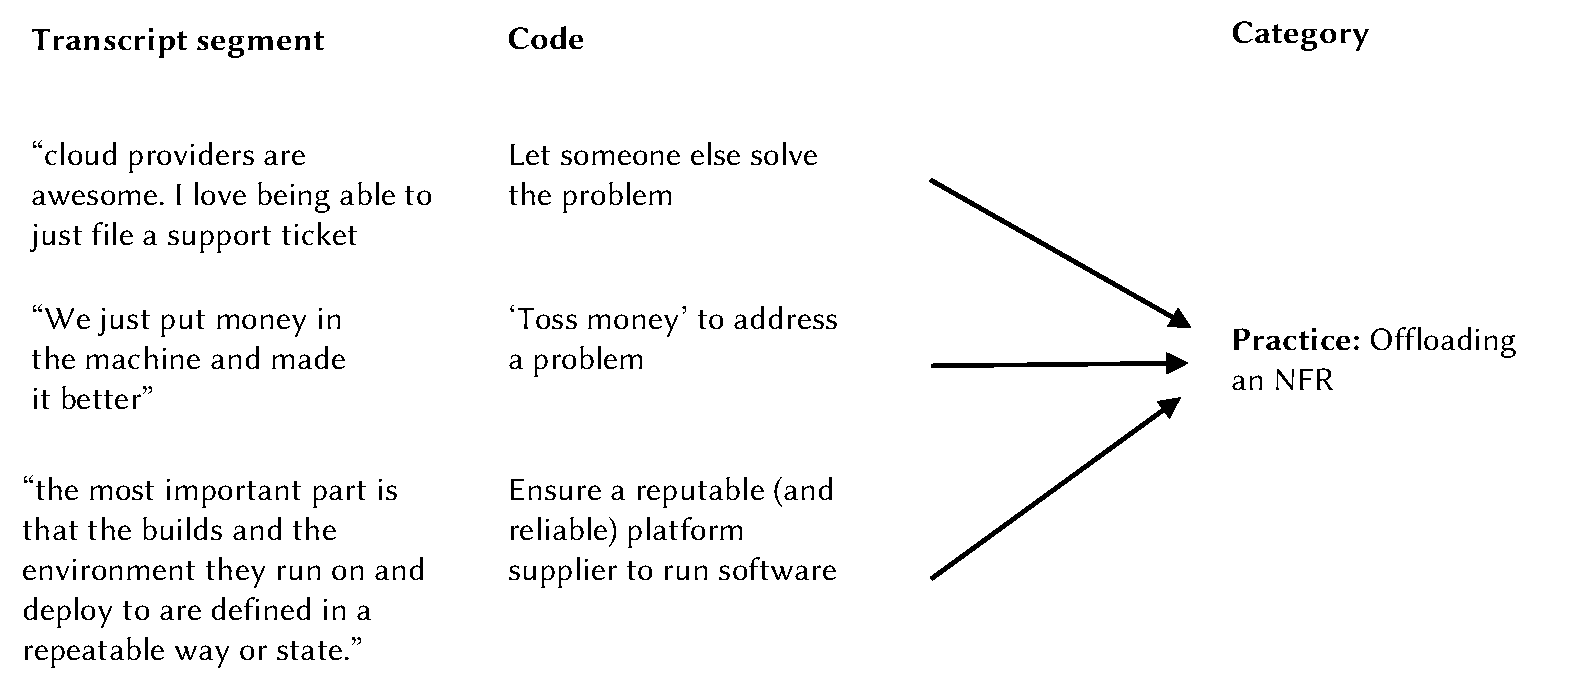
\includegraphics[width=12cm]{colin-coding-example.pdf}
    \caption{Example of coding}
    \label{fig:codingexample}
\end{figure}



We used member checking as a practice to establish the validity of our analysis. We used a short online survey to check whether our intermediate analysis findings resonated with the informants 
which presents intermediate findings through an online survey. Based on the feedback, we abandoned some themes that did not resonate with participants and made further amendments as our analysis continued. 

\subsection{Shaping Propositions}
As our analysis continued towards the development of propositions, we also identified links between different categories. We used practices akin to what \citet[p. 96]{strauss1990basics} labelled axial coding; that is, ``making connections between categories.'' This process involves asking questions about the phenomenon that we observed (e.g. ``what is the action/interaction all about?'' \cite[p. 100-107]{strauss1990basics}), causal conditions that led to the phenomenon, and consequences or outcomes of the phenomenon. During this process, we captured our observations and deliberations in short memos. Table~\ref{tab:samplecode} shows an excerpt of this process. For example, we identified `loss of control' as a potential consequence of the practice of `offloading an NFR'; a lack of shared understanding as a consequence of de-prioritizing NFRs, and a service disruption as a manifestation of a lack of shared understanding.
Part of these analysis procedures was the sketching of our emergent propositions and identifying links among categories \citep{eisenhardt1989building,miles1994qualitative}. Ultimately, the development of these propositions is subjective, insofar that different investigators are likely to come up with an alternative interpretation, because each investigator has a certain background and experience which naturally influences their interpretation and ability to identify patterns. We discuss our positionality below, and discuss the inherent subjectivity of the analysis process as a threat to validity.

\begin{table}[!bt]
\caption{Identifying relationships among concepts: antecedents and consequences}
\label{tab:samplecode}
\footnotesize 
    \begin{tabular}{p{4cm}p{4cm}p{3cm}}
    \toprule
    Transcript segment & Memo & Theme \\ \midrule


    ``Availability is actually an interesting one, do you spin up Amazon services in Virginia, or do you avoid that because that's their biggest region and so things sometimes go wrong there.'' (Alpha) 
& Manager talks about how they become reliant on a cloud provider to provide an NFR, but they are also at the mercy of the cloud provider, resulting in a loss of control over that NFR. &  Offloading an NFR is \emph{susceptible} to loss of control \\
    \addlinespace
    

    ``It's a scalability issue, but it's not prioritized, so we need to build more domain knowledge so it doesn't fall by the wayside.'' (Beta) & Developer and manager indicate that scalability was an issue, but was not a high enough priority due to a lack of shared understanding. & Deprioritization \emph{results in} lack of shared understanding \\
    \addlinespace

    ``The developers working on the code didn't know the impact causing an outage, this is one of those things that people don't pay too much attention to until they need to.'' (Gamma) & A lack of shared understanding of transparency resulted in a loss of service for a customer. & Lack of shared understanding \emph{manifests as} a service disruption \\    
    
    \bottomrule
    \end{tabular}
\end{table}

After analyzing the data from cases Alpha, Beta, and Gamma, we established initial propositions that together formed an emergent process theory. This emergent theory was then further refined as we collected and analyzed data from the fourth case study at Delta. At this point, we engaged in what \citet[p. 108-111]{strauss1990basics} described as ``verification of statements against data'' and ``a constant interplay between proposing and checking.''
This entailed an iterative process of adding and refining statements to the emergent theory, while ensuring that prior statements remained valid as new insights were generated. 
The fourth case study, therefore, served the purpose not only of verification of the initial set of propositions but also to add further nuance to the emergent theory. For example, a key contribution of the case study at Delta was our observation that certain practices were used proactively to build a shared understanding of NFRs (see Proposition 3, discussed later), something we had not observed in the first three case studies.
To illustrate the refinement process: Table~\ref{tab:proprefinement} shows an early version of Proposition 2, and of Proposition 3, which originated in insights gained from the fourth case study.
Upon closer inspection of the practices that we identified, we observed that the practices that were use in response to a trigger appeared categorically different in nature than those that were used proactively. The former allowed developers to manage, monitor, or quantify an NFR, and so we called these  `management' practices. The latter, on the other hand, appeared to focus on information exchange, and so we called these communication practices. This distinction then led to the refinement of these propositions.


\begin{table}[!t]
\caption{Example of refining propositions}
    \label{tab:proprefinement}
    \centering
    \begin{tabular}{p{2cm}p{4cm}p{5.3cm}}
\toprule
Proposition & Earlier version & Final version \\
\midrule 
Proposition 2 & A trigger prompts an organization to implement a practice to build shared understanding of a non-functional requirement.     &   Management practices are primarily used to reactively build a shared understanding of non-functional requirements, in response to triggers.\\
\addlinespace
Proposition 3 & An organization may also implement a practice unprompted.  & Communication practices are primarily used to proactively build a shared understanding of non-functional requirements. \\
\bottomrule 
\end{tabular}    
\end{table}



\subsection{Positionality of the Investigators}
We now briefly discuss the positionality of the investigators. 
The lead author has worked in the software industry for almost 20 years. He is currently a Director of Engineering, and has previously worked as an operating system specialist and software developer. He holds a PhD in Computer Science. His experience of having worked in both large and very small companies has influenced his vision on software engineering as a practice, but also as a field of research. The second author has worked in the IT industry for 10 years in varying roles. She holds a Master's degree in Computer Science. 
The third and fourth authors are professors of software engineering, and both have primarily an academic focus on research. Both have extensive experience in conducting fieldwork, qualitative data analysis, and theorizing (cf. \citep{damian2002impact,stol2014key}). 

\section{The Ebb and Flow of Shared Understanding of Non-Functional Requirements in Small Organizations using Continuous Software Engineering}
\label{theory_overview}

We now present the results of our theory development, which comprises six propositions. For each proposition, we juxtapose suggestions, findings, or assumptions from prior literature, with the findings from our fieldwork. 
We present a visual presentation of the theory in Figure~\ref{fig:iceberg}.


\begin{figure}[!h]
    \centering
     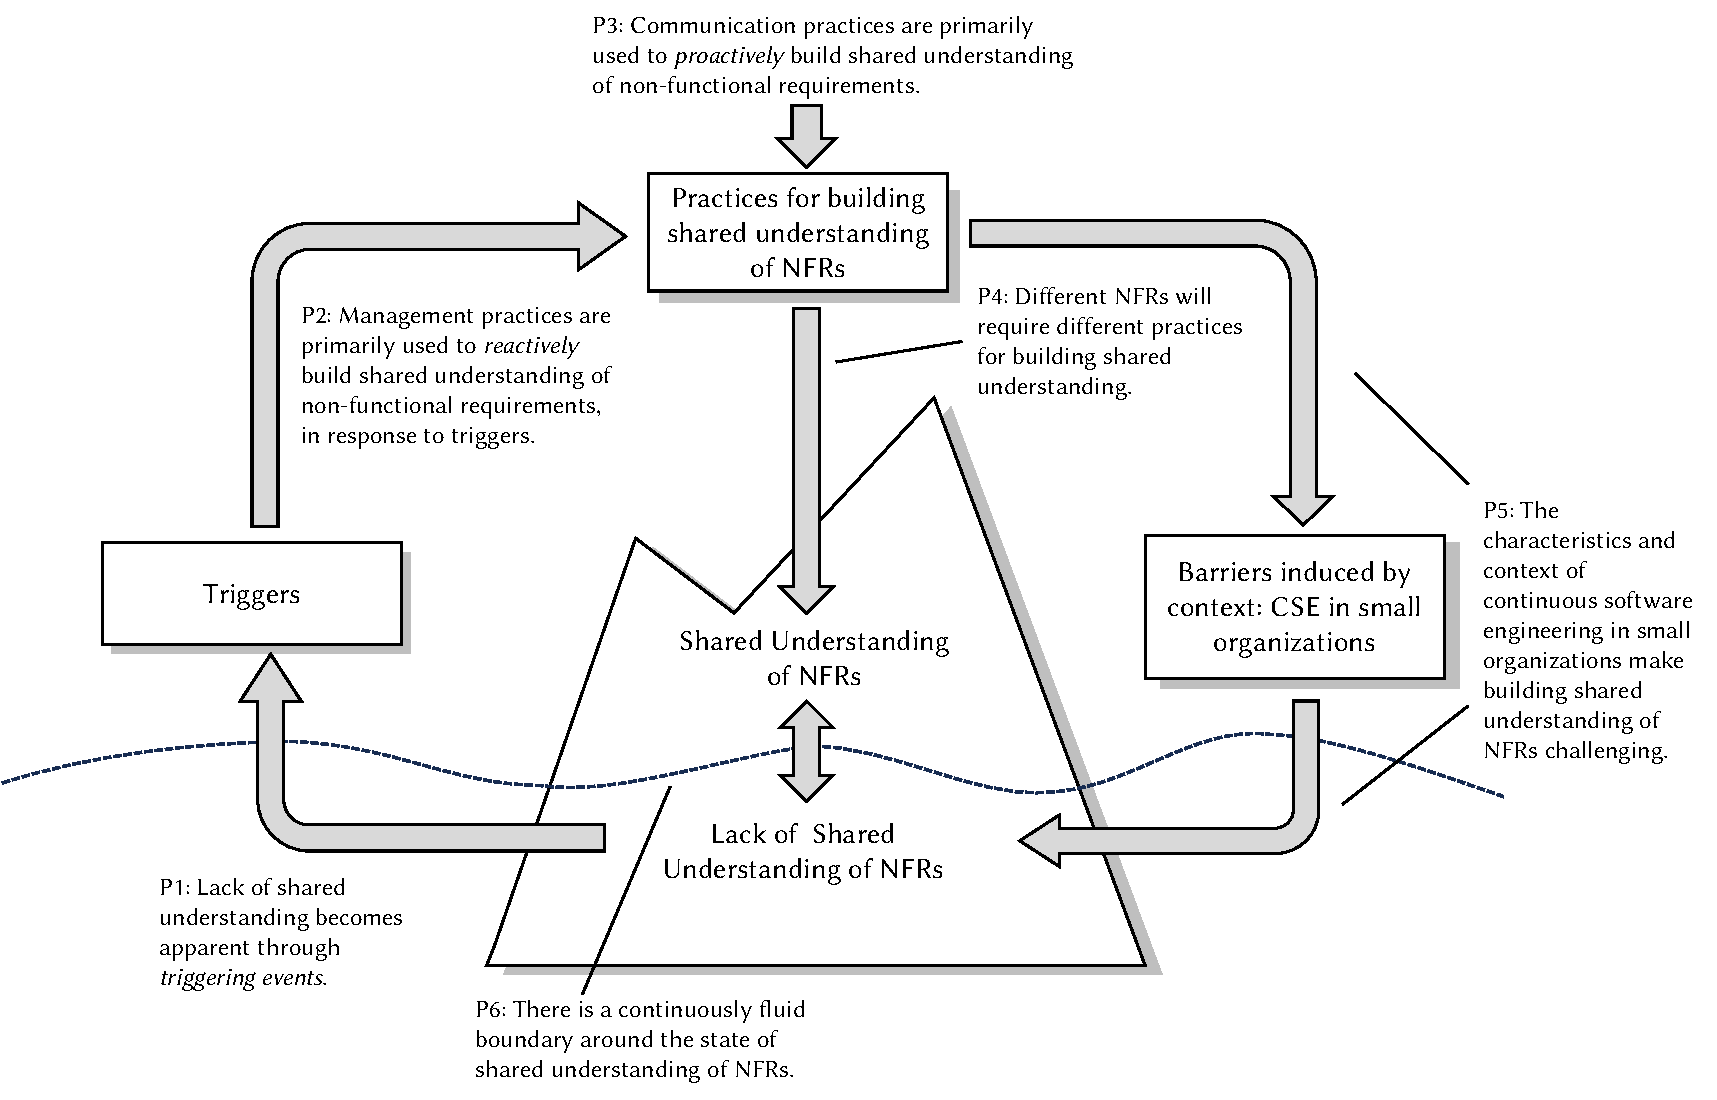
\includegraphics[clip,trim={0 0 0 0},width=12cm]{icebergtheory-11sep24.pdf}

    
    \caption{The Iceberg theory of managing shared understanding of non-functional requirements in continuous software engineering contexts}
    \label{fig:iceberg}
    
\end{figure}

\subsection{Detecting Lack of Shared Understanding of Non-Functional Requirements}

How might a lack of shared understanding manifest or be detected?
\cite{glinz_shared_2015}'s taxonomy suggests that shared understanding is either true or false: either members of a team share an understanding (i.e., a true shared understanding), or they believe they have a shared understanding, but in actual fact, they do not (i.e., a false shared understanding). 
To determine whether a group of people have a shared understanding, \cite{glinz_shared_2015} identified and discussed 11 practices. For example, to create and play out scenarios to evaluate whether everybody understands how a system will work in these given scenarios. 
There are two potential issues with this set of practices. First, they cannot \textit{necessarily} identify a \textmd{specific} lack of shared understanding of a given topic or part of a system. Second, and perhaps more importantly, most practices appear to assume that a team \textit{proactively} performs these practices to establish whether there is a shared understanding. 

The findings of our field study suggest that a lack of shared understanding is not proactively assessed, but instead is revealed through emergent critical events. 
We call these `triggering events' (or `triggers' for short \citep{werner2020re}), which make team members aware that there is a lack of shared understanding of an NFR. Or, formally stated:

\cwproposition{1}{A lack of shared understanding of non-functional requirements becomes apparent through triggering events.}

Table~\ref{tab:triggers} presents data that grounds this proposition. In all cases, we found that there are triggers that led to a team's realization that they lacked a shared understanding of specific NFRs. 
Our analysis revealed five categories of triggers, though it is likely that these are not exhaustive. We elaborate on these categories below.\footnote{The set of triggers presented here is a revised set of categories after we initially reported these in \cite{werner2020re}.}

\begingroup
\footnotesize 
%\small 
\begin{longtable}{P{1.5cm}p{4.8cm}p{3.3cm}p{1.3cm}}
\caption{Categories of triggering events and selected examples}\label{tab:triggers}\\
    \toprule
    Category  & Example & Description & Company \\
    \midrule
\endfirsthead
    \multicolumn{4}{l}{\textbf{\textsf{Table~\ref{tab:triggers}}}\hspace{2mm}Categories of triggering events and selected examples (continued)}\\
    \addlinespace 
    \toprule 
    Category  & Example & Description & Company \\
    \midrule
\endhead
   \bottomrule
\endfoot
    \bottomrule     
\endlastfoot



New \newline requirements  
& ``So they wanted to extend it and could not figure out how without doing all this rework to start with.''
& Lack of knowledge was revealed when new requirements are to be implemented.
& Alpha\\

\addlinespace 

%New Requirements  
& ``You might get halfway through implementation and realize there are a whole bunch of questions that you don't know the answers to. And those questions should have been answered but weren't, either because no one understood at the time or because you've discovered new requirements.''
& Questions arose during implementation, identifying new requirements. 
& Delta\\

\addlinespace

& ``something out of our control changed, or other things have changed since that was put into place due to privacy regulation acts'' & Privacy regulation as a source of new requirements. & Gamma\\

\addlinespace

% Customer demands  
% &
% ``if a lot of customers had this setup, then [the priority] would have been high''
% & High priority rework task
% & Alpha\\

% \addlinespace


Customer demands  
& ``[this issue was a] big problem for one user, one very big user, because for [redacted customer's name] everything that company says is critical.'' 
& An NFR-related issue became a high priority rework task when an important customer reported it.
& Beta\\

\addlinespace

%Customer demands  
& ``if your requirement is still the same and your system is still working as it was, but it's the actual environment that has changed.''
& The customer's environment differs from the development environment, highlighting an issue e.g. portability. 
& Gamma\\

\addlinespace

Technical debt  &
``any time you needed a place to put something we used to toss them on that big stack of
unorganized classes until it became a giant object.''
& Lack of shared understanding regarding the trade-off between taking on technical debt and maintainability. A lack of shared understanding led to continued behaviour, ultimately requiring very significant rework. 
%Need to refactor code, after an initial lack of shared understanding of maintainability
& Beta\\

\addlinespace

%Technical debt 
& ``two people [developing] independently, they talk to each other well, but you’re still going to approach problems differently and hit different areas of the system and not know everything that’s going on.''
& Misunderstandings become clear as developers discuss how to refactor code to address technical debt.
& Beta \\

\addlinespace

Scope creep 
&
``start an app early on for North American companies requiring one [format]. As your app becomes more popular you start getting requests for new countries that use [other] formats'' 
& Lack of shared understanding of configurability.
&  Gamma\\

\addlinespace

%Scope creep  
& ``they had made the assumption that they would be able to go in and update these prints after launch. And we had made the interpretation that everything was just sort of hard-coded, write once and forget it. And so, in the end, it was something that we actually had to push back on the client and say that, making that something that’s editable, would significantly increase the scope.''
& Need for major rework to make a system that is more flexible that had not been foreseen.
& Delta\\

\addlinespace
Service disruption &
``The rework on it was not only to refactor it [...] but essentially to handle the type of
structure used [in the application] that caused problems throughout the app.''
& An NFR-related issue caused considerable rework due to what turned out to be a lack of shared understanding.
& Alpha \\



\end{longtable}
\endgroup 

\paragraph{New requirements} The first category of triggers is the emergence of new requirements: during design and implementation discussions, developers may realize that parts of the design were not sufficiently specified. For example, at Alpha, some functionality had to be extended, and developers were unclear as to how to achieve this without considerable rework. The discussion among developers led to the realization that they lacked a shared understanding.
Many NFRs are driven by a specific business domain; for example, performance was key to three of the four organizations we studied (see Table~\ref{tab:companies}). Other NFRs may emerge due to regulation; for example, the 
GDPR mentioned earlier, came into effect in 2016, and requires that organizations collecting or processing data in the EU must comply with specific privacy regulations. This, too, imposes new requirements which may lead to the realization that teams lack a shared understanding of how to implement such privacy requirements.

\paragraph{Customer demands} We identified a second category of triggers that we labelled `customer demands.' On occasion, customers would offer feedback, reporting problems with NFRs such as performance. This would then lead to an investigation of the issue, and a realization that the team did not share an understanding of a specific NFR.  For example, at Beta, a problem emerged due to poor performance in the system deployed to one major customer. Escalation of the issue would depend on the scale of the problem, but also the customers affected. Or, as a developer at Alpha mentioned: \textmd{``if a lot of customers had this setup, then [the priority of the issue] would have been high.''}


\paragraph{Technical debt} A third category of triggers is issues arising due to technical debt. For example, a lack of shared understanding of maintainability for a product at Beta caused issues because developers writing new functionality would simply ``toss them on that big stack of unorganized classes until it became a giant object.'' While the initial developer, who placed new functionality in a `utility' component or class without proper integration into a coherent architecture, may have made a conscious decision to trade-off technical debt against maintainability,  this action had consequences. This initial action served as a precedent for other developers to continue this practice without consciously acknowledging the trade-off that had been made earlier. 
Ultimately, this `snowballing' of continuing to follow initial precedent led to problems affecting the whole app,
%``throughout the app,'' 
meaning that considerable rework was necessary. Developers would try to resolve defects, but in actual fact, they were exacerbating the overall technical debt. This would continue until such time that a decision was made to address the underlying issue and undertake a major refactoring. To perform the refactoring, however, developers now had to come to a shared understanding of how to improve the maintainability, and redesign parts of the application. 

\paragraph{Scope creep} A fourth category was labelled scope creep, which has been defined as ``the growth of the scope of a project's requirements beyond those originally intended'' \citep{williams2009exploring}. In this context, the growth of scope related to NFRs arose due to an initial lack of understanding of the requirements. For example, at Gamma, an initial version of the system under development focused exclusively on the North American market, with its specific standards, notations, and customs. Only when the team was instructed to deploy the system to other countries (with different standards and notations), was a lack of shared understanding of the need for configurability detected. 

\paragraph{Service disruption} Finally, a fifth category of triggers is service disruption; triggers in this category refer to critical events that interrupt the software from working correctly, due to a lack of shared understanding of NFRs. For example, a lack of shared understanding of scalability turned out to be a major problem at Alpha, leading to a service disruption. A developer at Alpha explained that, rather than refactoring the code, to prevent future breakdowns, it had to be redesigned to \textmd{``handle the type of structure used that caused problems throughout the app.''}


Why does a lack of shared understanding get detected through triggering events, rather than proactive assessment by teams?
One reason may be that many practices that can help to assess shared understanding are based on explicit documentation or artifacts \citep{glinz_shared_2015} and that assessment activities such as 
creating and playing scenarios, model checking, and comparing to reference systems \citep{glinz_shared_2015}, 
all require teams to proactively allocate time to perform these activities and capture the information that is gathered. In small companies, in particular, such resources may not be available.

A second reason may be the pressure to keep delivering new versions of the software in CSE settings. Many of the practices in CSE can be linked to `Lean Thinking' \citep{fitzgerald2017continuous}, emphasizing minimizing waste, which means removing unnecessary activities and not creating unnecessary artifacts. We found no evidence in our fieldwork of any proactive attempt to assess or identify a lack of shared understanding of NFRs. 
Further, our focus on small organizations, all of which started as startups about 10 years before we conducted our fieldwork, underscores this. The Lean Startup movement, itself influenced by principles of Lean Thinking \citep{ries_lean_2011}, emphasizes reducing the time between a feature request and `cash' \citep{fitzgerald2017continuous}. 

Finally, practices to proactively assess a lack of shared understanding do not appear to focus on any specific NFR. All data collected in this study suggest that a lack of shared understanding is only realized when problems with a specific NFR occur. For example, reliability turned out to be poor for Alpha when their service was disrupted. Performance turned out to be poor for Beta when an important customer reported problems that required urgent attention.
While practices for proactively assessing a lack of shared understanding could work in general, they lack focus on specific NFRs.








\subsection{Building Shared Understanding of Non-Functional Requirements}


How might developers \textmd{build} a shared understanding of NFRs in CSE settings? 
Prior literature suggests a number of enabling practices to build shared understanding \citep{glinz_shared_2015}. Glinz and Fricker argued that these practices can \textmd{``constructively [lower] the probability of undetected misunderstandings.''} Practices as reported in prior literature can be effective in sharing knowledge and building a shared understanding of requirements, including NFRs. However, our study offers a more nuanced account of how organizations manage a lack of shared understanding of NFRs. We found that organizations do not necessarily proactively invest in building a shared understanding of NFRs, but that they do so in response to certain critical triggering events, discussed earlier. 
Drawing on insights from the general requirements engineering and knowledge-sharing literature, \citet{glinz_shared_2015} identified several practices for enabling and building shared understanding in general. Enabling practices include activities such as team building, collaborative learning, negotiation, and prioritization. Building practices include activities such as modelling, creating glossaries and ontologies, prototyping, workshops and handshaking \citep{glinz_shared_2015}. 

While NFRs are a particular type of requirement, the literature has been quiet on how a shared understanding of NFRs, specifically, is developed. Much of the state of the art, as compiled by Glinz and Fricker, is presented as a set of unproblematic practices that can be performed without any issue. The findings of our study offer new insights into this. 
First, we distinguish between what we label \textmd{`management'} practices and \textmd{`communication'} practices. Management practices include activities that allow the measurement and monitoring of NFRs and are primarily invoked in response to triggers. In contrast, communication practices include activities that leverage interaction between developers and other stakeholders to clarify NFRs and are primarily used to build shared understanding proactively. Thus, more formally, we posit:

\cwproposition{2}{Management practices are primarily used to reactively build a shared understanding of non-functional requirements, in response to triggers.}


\cwproposition{3}{Communication practices are primarily used to proactively build a shared understanding of non-functional requirements.}
%
Further, we also found that different practices are likely necessary for building a shared understanding of different NFRs. Hence, we add:

\cwproposition{4}{Different non-functional requirements require different practices for building shared understanding.}


\noindent Table~\ref{tab:practices} presents data from the fieldwork, organized by the practices that we distilled.\footnote{Table~\ref{tab:practices} presents a revised set of practices that were previously reported in \cite{werner2020re,werner_tse_2021} and \cite{okpara_re2022,okpara_rej2023}.} We note the specific NFR that was the topic of discussion or indicate `all' if the description is generally applicable. Each practice is labelled as either a management or communication practice.
We discuss evidence for Propositions 2, 3, and 4 in Sections \ref{sub:management}, \ref{sub:communication}, and \ref{sub:different}, respectively.



\begingroup
\footnotesize 
%\small 
\begin{longtable}{P{1.2cm}p{3cm}p{3cm}P{1.4cm}p{1.6cm}}
\caption{Evidence for Propositions 2, 3, and 4: Practices for building Shared Understanding of NFRs}\label{tab:practices}\\
    \toprule
    Practice & Example & Description & Company / NFR & Practice type \\
    \midrule
\endfirsthead
    \multicolumn{5}{l}{\textbf{\textsf{Table~\ref{tab:practices}}}\hspace{2mm}Evidence for Propositions 2, 3, and 4 (continued)}\\
    \addlinespace 
    \toprule 
    Practice & Example & Description & Company / NFR  & Practice type \\
    \midrule
\endhead
   \bottomrule
\endfoot
    \bottomrule     
\endlastfoot

%Put a number on the NFR 
% Quantifying the NFR
% & ``I think quick feedback is the core of DevOps so that we will see what broke [and] it reduces risk because things are integrated more frequently.''
% & Beta; reliability & Management\\

% \addlinespace 

% & ``developers really want [the] feedback loop to be tight.'' & Beta; reliability\\

% \addlinespace 

% & ``the good thing about developing at Delta is that our loops are pretty quick; we have a lot of communication, so it becomes quite clear when something isn’t being met.'' & Delta; performance\\

% \addlinespace

Quantifying an NFR & ``a certain amount of monitoring set up [...] You’re also defining which alarms are set. Therefore, if requests [drop] below [redacted] milliseconds and that’s what you want to hold it to. Then that would be codified in the alarm'' 
& Monitoring infrastructure and continuous monitoring help to establish baselines and thresholds that assume `meaning' among developers, who will establish a shared understanding of how to interpret these numbers and what actions might have to be taken. 
& Alpha; scalability & Management\\

\addlinespace 


& ``that 90\% of our customers have less than [redacted] items [...] They’ll [say] we know that each [order] requires [redacted] page loads'' 
& Quantification allows establishing trends across different customers, which means that variables such as `page loads' now convey meaning among team members. 
& Beta; performance 
& \\

\addlinespace 

& [tracked through a] ``[caching ratio] that we have from [redacted] our caching provider goes [on a dashboard] because that’s usually a pretty good indication that something has gone wrong. It also drastically affects performance.'' 
& The caching ratio in the application is an indicator of performance; quantifying and displaying this number will help establish a common understanding among the team of when something might be going wrong.
& Gamma; performance 
& \\

\addlinespace
%\newpage 



% & ``showing how many users are using a specific feature, where the feedback benefits developers but our product team in their ability to make their decisions''  & Gamma; \\

% \addlinespace

%%%%Let someone else manage the NFR 

% Offloading the NFR
% &
% ``[your web application is] immediately spread across however many availability zones and nodes as you want'' & Alpha; scalability & Management \\

% \addlinespace

% &``For anything that I do, [infrastructure as code] ends up in Terraform as a form of
% documentation'' & Alpha; configurability \\

% \addlinespace

Offloading an NFR & ``the most important part is that the builds and the environment they run on and deploy to are defined in a repeatable way or state.'' 
&
To offload an NFR, 
To offload an NFR, appropriate configuration scripts must be written; the process of developing such scripts requires an agreement on that NFR at that point, hence it temporarily contributes to building shared understanding of that NFR.
& Alpha; reproducibility 
& Management \\

\addlinespace

& ``cloud providers are awesome. I love being able to just file a support ticket'' 
& Offloading NFRs such as reliability requires some shared understanding to design the software to work with the cloud provider in the first place.
& Beta; reliability\\

\addlinespace

% & ``It automatically does it in the Docker compose files. So we've automated a lot of dependency updates and stuff like that'' & Beta; performance \\

% \addlinespace

& ``We just put money in the machine and made it better'' 
& To increase performance, more compute resources can be acquired from a cloud provider, but the software must be designed to allow this scalability. To achieve this, a shared understanding of NFRs such as performance must be achieved first. 
& Gamma; performance\\

\addlinespace

%Write your own tool 
\multirow[t]{4}{=}{Develop custom tools and standards}
& 
``If you want to change our usability parameters or whatever we change it in the source code and then we can test it and verify that it still meets our needs'' 
& Development standards and tools may include templated solutions, or simply the codification of key variables of interest as parameters; the code and interpretation of these parameters are visible to the team to help build shared understanding. 
& Beta; usability 
& Management\\

\addlinespace


& 
``so we used to have [redacted commercial offering] dashboards out there ... [but that] didn't give us any application-specific information'' 
& Developing a custom support tool focuses on domain-specific metrics as opposed to basic metrics (CPU, memory, etc). These domain-specific metrics are then published in source code and dashboards to facilitate building a shared understanding.
& Gamma; performance & \\

\addlinespace


& ``I introduced a number of standards and built some packages to try and enforce those
standards. So there’s the standard for how we, on the server side, get configuration from
the environment'' 
& Developing custom libraries or standards implies that all team members must learn these as agreed upon `protocols', implying that a shared understanding is built.
& Delta; maintainability & \\

\addlinespace

% & ``so there’s a lambda [function] that runs when you make a bucket, it triggers and goes `you didn’t encrypt’, it turns on encryption, tells you, `you are an idiot'. Security non-functional requirement!”  & Alpha; security \\

% \addlinespace


%Put the NFR in source control
Capturing an NFR in version control
& 
``with respect to codifying something vs documenting it: it’s not precise enough it’s written in English. It’s open to interpretation'' 
& Capturing NFRs in natural language lacks precision which may cause decay of shared understanding. Establishing exact threshold or cut-off values allows for an unambiguous definition of NFRs, contributing to a shared understanding.
& Gamma; configurability 
& Management \\

\addlinespace

Solicit feedback & 
``there are things like code review, review and feedback from the managers that sort of catches the NFRs'' 
& Feedback comes from different sources including code review, colleagues and managers. Such feedback may incorporate clarification contributing to a shared understanding among team members.
& Delta; maintainability 
& Communication \\

\addlinespace

& ``our [deep-dive] during the development process and the project engineering role really
helped with that. Because when the shaping is happening, we’re starting to think about those non-functional requirements: how it might work for other use cases, how something should be developed from a quality perspective and what tools we are using'' 
& Feedback during a deep-dive meeting helps to clarify NFRs, thereby contributing to a shared understanding of these NFRs.
& Delta; usability & \\

\addlinespace

%\newpage 

Leverage past experience 
& 
``I think the biggest tool that has helped me learn NFRs has really just been reviewing previous work, specs, and integrations.''  
& Discussing how NFRs were previously implemented helps build a shared understanding among the team. 
& Delta; all 
& Communication \\

\addlinespace

& ``there’s a process that isn't formally presented, it’s picked up over time through training. I think that the majority of NFRs have been picked up that way''  
& Training over time helps build shared understanding of NFRs.
& Delta; all 
&\\

\addlinespace

Wireframing 
& 
``something like Figma or Figjam to quickly visualize what we're talking about.'' 
& Visualizing as a form of prototyping helps to build a shared understanding of a system's usability.
& Delta; usability 
& Communication \\

\addlinespace

& ``that’s where things like `shaping,' wire-frames, starting to try to think through that user experience really helps. Design drawings, I find are really helpful. Early mock-ups help people because I find that a lot of the team does well with actually experiencing something.'' 
%%They quickly start to see this does the thing, but it’s totally unusable for other reasons.''
& 
Creating mock-ups helps a team of developers to ``experience'' a system as if they were users, thereby creating a shared undersatnding of usability.
& Delta; usability 
& \\

\addlinespace
%\newpage 

%%Discussing problems and solutions 
\multirow{2}{=}{Knowledge sharing activities} 
& 
``it’s been helpful for talking about how we build things and non-functional requirements in specific areas of our jobs'' 
& Facilitating organized opportunities (e.g. `guild' meetings) to share knowledge on for example implementation, helps to build shared understanding of NFRs. 
%For example, so-called `guild' meetings are scheduled meetings to bring together team members to discuss how NFRs are implemented.
& Delta; all 
& Communication \\

\addlinespace 

& ``Great user experience is one of those things that’s difficult. When it comes to user experience, we've centralized the people who make user experience decisions into a group and then we have standards in that group'' 
& Bringing together all people involved in system user experience helps to share and codify relevant knowledge.
& Delta; usability 
&\\

\addlinespace 

Asking questions 
& 
``you want to ask a lot of questions, you want to poke a lot of holes and things and, really
go to the very edge of, you know, when you’re sketching it out.'' 
& 
While knowledge sharing activities are useful to develop a shared understanding of `known' knowledge, what others have called `unknown unknowns' are harder to share. Asking questions is a complementary practice to probe and explore some knowledge that might otherwise not be shared, because it was unknown, unthought of, or tacit in nature. 
& Delta; all 
& Communication \\

% \addlinespace 

% & ``when we go into the deep-dive, we know when the non-functional requirements have been met when we as a group meet, and there aren't gaps in our shared understanding. We come out of a review meeting, and there’s not a lot of feedback'' 
% & \hl{Colin, this example seems to link closely to the 2nd example given for `solicit feedback' (mentioning deep-dive). } \hl{Klaas, agreed. Should we remove?}
% & Delta; all 
% &\\


\end{longtable}
\endgroup 



\subsubsection{Management Practices}
\label{sub:management}
The first set of practices is classified as management practices, so called because they allow developers or teams to manage, monitor, quantify, and make an NFR explicit. 

\paragraph{Quantifying an NFR} A first management practice is quantifying an NFR, which is a management practice because the ability to do so allows an organization to assess, validate, and monitor the NFR over time. This, in turn, creates a feedback loop in the form of information about how the system performs in terms of NFRs, which feeds back into the development cycle. Quantifying NFRs as a practice is consistent with \citet{wagner2019status}'s finding that approximately half of the respondents to their large-scale survey used ``quantified textual documentation for non-functional requirements.''
At Beta, the CSE approach enabled a fast feedback loop, which allowed a quick detection of defects causing system crashes, as one developer described: 
\textmd{``I think quick feedback is the core of DevOps so that we will see what broke [and] it reduces risk because things are integrated more frequently.''}


The feedback loop is most useful if it is \emph{fast},  and many organizations strive to reduce the time required for a feedback loop to complete. 
Quantifying an NFR is typically done with dashboards that help with the proliferation of shared understanding of those monitored NFRs.
A dashboard may be shared across an entire organization, stretching beyond the barriers of the development team, as all units of an organization, from finance to marketing, embrace the `continuous *' approach \citep{fitzgerald2017continuous}.

Many organizations use metrics to monitor common NFRs, such as availability, performance, scalability, availability, and reliability \citep{werner_tse_2021}.
For Gamma, performance is a vital NFR and is tracked through a caching ratio retrieved from a caching provider, and captured on a dashboard, said one developer:
\begin{quote}
``[the caching ratio] that we have from [...] our caching provider goes [on a dashboard] because that's usually a pretty good indication that something has gone wrong. It also drastically affects performance.''    
\end{quote}


\noindent We found a similar setup at Alpha, as one manager explained how warnings and alarms are based on thresholds:
\textmd{``if requests [drop] below [a certain number of] milliseconds and that's what you want to hold it to. Then that would be codified in the alarm.''}
At Delta, performance is primarily monitored through Datadog \citep{data_dog}, a commercial cloud-based monitoring offering; metrics such as error rates, average response times for API calls, and number of application instances are indicative measures of the state of their systems and applications. 

Some NFRs are easier to quantify than others. As \citet{wagner2019status} observed, performance is more easily quantified than, for example, maintainability.
One way for an organization to continuously validate usability is through iterative end-user testing or behavioural testing with stakeholders, by leveraging tools that support behavior-driven methodology. 
A manager at Beta explained how they use this approach to determine, for example, that 90\% of their customers have less than a certain number of products in their basket, and that each order requires a certain number of page loads, in turn affecting usability. The page load count is, therefore, a variable that can be used in the design and development of a product basket, and to assess how usability might be affected. 
At Gamma, we found metrics to play a key role in managing usability across cross-functional teams, including development and product management, as one developer explained:
\textmd{``showing how many users are using a specific feature, where the feedback benefits developers but [also] our product team in their ability to make their decisions.''}
Additionally, monitoring usability may be accomplished by embedding components in the user interface that report statistics back to the organization, enabling the organization to understand how their software is being used, what features are and are not being used, and how efficient their user interface is to use.


\paragraph{Offloading an NFR} A second management practice is offloading an NFR, which we found to be the most common approach among the small companies that we studied. 
Small companies tend to be more resource-constrained than large organizations, which means that they may need to set stricter priorities in terms of the NFRs they focus on. Offloading NFRs that have a lower priority allows small companies to do so. 
Offloading an NFR allows an organization to effectively ``ratchet'' \citep{bellomo2014}, as a manager at Gamma concisely described: \textmd{``we just put money in the machine and made it better.''}
Ratcheting allows an organization to consume more cloud provider resources or access locked features to handle a particular NFR bottleneck.

In practice, offloading an NFR can imply the use of configuration scripts, or Infrastructure as Code (IaC), to facilitate the bridge to cloud providers. This means that, while the NFR itself, such as availability, can be `secured' as the company now uses compute resources available with cloud providers, there is still a need to gain a good understanding of how the NFR can be achieved and implemented in terms of making appropriate configurations. It is this process that helps in building a shared understanding of the NFR. 


Many NFRs, such as availability, scalability, and reliability, can be offloaded either entirely or partially, typically to a cloud provider.  
Cloud providers also offer support when issues arise. A developer at Beta described this succinctly: \textmd{``cloud providers are awesome. I love being able to just file a support ticket.''}
For example, a manager at Alpha explained the benefit of offloading to achieve scalability, without the need to invest in resources such as in-house hardware:
\textmd{``[your web application is] immediately spread across however many availability zones and nodes as you want.''}



Offloading NFRs is a viable tactic, particularly in CSE contexts. CSE emphasizes automation, including the development and deployment environments; such IaC increases configurability in general, and this, in turn, reinforces the benefits of CSE approaches \citep{humble2010continuous}.
IaC has grown to capture more quality aspects of software, including build, staging, and deployment infrastructure, with very little input required from humans \citep{humble2018accelerate}.
A manager at Alpha described how IaC scripts capture the configuration:
\textmd{``For anything that I do, [infrastructure as code] ends up in Terraform as a form of documentation.''} 
Besides improving configurability, it also enables organizations to codify other NFRs captured as IaC. 
A developer at Beta described how the complexity of the system becomes more maintainable:
\textmd{``it automatically does it in the Docker compose files. So we've automated a lot of dependency updates and stuff like that.''}



\textbf{Custom tools and standards.} A third management practice is developing custom tools and standards. 
Off-the-shelf solutions may not satisfy an organization's specific needs and may need some heavy modifications, as one developer at Gamma pointed out:
\textmd{``so we used to have [tool name] dashboards out there ... [but that] didn't give us any application-specific information.''}
We found that companies use custom tools, or customize existing tools, to enforce specific NFRs. 
For example, Beta and Gamma each codified certain usability parameters in their source code, leaving no room for misunderstandings. That way, the results of any changes can be observed after the committed changes have propagated through the CSE pipeline, as one developer at Beta described:
\begin{quote}
    ``If you want to change our usability parameters or whatever, we change it in the source code and then we can test it and verify that it still meets our needs.''
\end{quote}    

\noindent At Delta, developers defined and shared development standards within packages and custom tools to define how some NFRs are managed. A manager at Delta described this:
\begin{quote}
    ``I introduced a number of standards and built some packages to try and enforce those standards. So there's the standard for how we, on the server side, get configuration from the environment.''
\end{quote}
Another example of a custom tool is a script that checks whether an agreed development standard to achieve security has been complied with, as a manager at Alpha described:
\begin{quote}
    ``so, there's a lambda [function] that runs when you make a bucket, it triggers and goes `you didn't encrypt,' it turns on encryption, tells you, `you are an idiot.'\,''    
\end{quote}


The decision on whether to write a custom tool or customize an existing tool comes with the question as to whether the effort involved can be sufficiently carried by the organization. This is particularly true if off-the-shelf or open-source solutions exist.

\paragraph{Capturing NFRs in version control} The fourth and final management practice that we identified is codifying and capturing an NFR in version control. 
Codification refers to capturing knowledge of NFRs in source code files and other artifacts, such as IaC configuration files, which can then be managed in version control systems.
Configuration for tools (including static analysis tools, code linters, and formatters) can be stored in source control alongside the source code.
The potential configuration of an NFR could include rules or triggers that represent thresholds for certain metrics that could trigger alarms or failures through a dashboard, or the CSE pipeline itself.



Codification helps set objectives for developers who might not have had enough time to gain the tacit knowledge about what constitutes an acceptable definition of an NFR.
Knowledge of NFRs may not be easy to communicate via natural language, as one developer at Gamma described:
\begin{quote}
    ``with respect to codifying something vs documenting it: it's not precise enough [if] it's written in English. It's open to interpretation.''
\end{quote}
Similarly, as for any requirement, NFRs must be specific, reducing any room for interpretation. For example, stating that ``the response time must be fast'' is not specific; instead, ``the response time must sub-100ms'' provides clarity that can be captured in source control. 


We found that the management practices we identified through this study were primarily used in response to some triggering event. That is, triggering events would reveal a lack of shared understanding, and if sufficiently severe, companies would take action to address it to prevent it from happening again. 
Why are these practices primarily used reactively, rather than proactively? 
One reason is that management practices, in general, tend to emerge due to an organization's realization and increased awareness. For example, \citet[p. 33]{gawande2010checklist}. described how the pre-flight checklist emerged in response to an airplane crash in 1935: the pilot had forgotten to conduct certain procedures in a relatively new airplane. The complexity of software development in a fast-paced CSE setting represents a challenging context for developers and other stakeholders to maintain a shared understanding. The management practices can be seen as `checklists,' activities and practices that address specific issues that had emerged at an earlier point in the project.
It is not until one has awareness of a problem, that it can be addressed.  
The practices described above therefore reflect a \textit{response} to an increased awareness. A proactive use of these practices would imply prior knowledge of problems before they would emerge. While some problems could be anticipated, it is more likely that issues with NFRs emerge only after initial implementation.


\subsubsection{Communication Practices}
\label{sub:communication}
A second set of practices to build a shared understanding of NFRs are communication practices. Proposition 3 states that these practices are primarily used proactively, without a triggering event. We discuss possible reasons why this is the case after we lay out the practices we identified.

\paragraph{Soliciting Feedback} The first communication practice we observed was soliciting feedback. Feedback activities such as code reviews and deep-dives as part of the CSE pipeline process, developers and other stakeholders can explain and clarify NFRs, and any issues or misunderstandings can be identified and addressed. A developer at Delta explained: 
\textmd{``there are things like code review, review and feedback from the managers that sort of catches the NFRs.''}
A code review is a common and proactive (i.e., not triggered by events such as those listed in Table~\ref{tab:triggers}) way to build a shared understanding of an NFR and also to solicit feedback that a given code contribution satisfies the expectations for some NFRs.
A thorough code review may reveal when 
expectations for an NFR have not been met. For example, code reviews can reveal the testability of a code unit, or when unit tests do not provide complete code coverage. 

Other types of feedback meetings such as deep-dives, also create opportunities for software teams to proactively build a shared understanding of NFRs.
Software developers can discover and initiate the shared understanding of NFRs as one developer at Delta explained: 
\begin{quote}
    ``our [deep-dive] during the development process and the project engineering role really helped with that. Because when the shaping is happening, we're starting to think about those non-functional requirements: how it might work for other use cases, how something should be developed from a quality perspective and what tools we are using.''    
\end{quote}
Software teams can use deep-dive meetings to demonstrate a product or a design, and subsequently discuss and verify that the product is aligned with both low-level requirements and high-level requirements.

A shaping meeting occurs at the start of a project where project stakeholders decide on the initial high-level requirements of a planned product. A deep-dive meeting, in contrast, occurs after project implementation begins, and usually includes only software developers or managers who are directly involved in the implementation. 
Continuously soliciting feedback on NFRs allows developers and other stakeholders to share and build knowledge regarding NFRs, contributing to a shared understanding.



\paragraph{Leveraging Past Experience} The second communication practice to build a shared understanding of NFRs is to leverage past experience. 
Previous projects may be reviewed, allowing developers to reflect and deepen their understanding of how NFRs were handled. Reflecting on past experience and discussing this is thus a communication practice.
A developer at Delta indicated this to be an important practice:
\begin{quote}
    ``I think the biggest tool that has helped me learn NFRs has really just been reviewing previous work, specs, and integrations.''
\end{quote}    

Unlike other communication practices, leveraging past experience was primarily a \textmd{reactive} practice; triggers such as technical debt or new requirements would encourage developers to address their lack of knowledge of the NFRs they focused on. However, this practice could also be undertaken proactively; for example, a developer at Delta described:
\begin{quote}
    ``there's a process [to learn about NFRs] that isn't formally presented, it's picked up over time through training. I think that the majority of NFRs have been picked up that way.'' 
\end{quote}    
An organization may proactively incorporate this practice in other processes such as the onboarding process, to have dedicated training and ongoing support \citep{sharma2020onboarding}.


\paragraph{Wireframing} The third communication practice we identified is wireframing, which includes the use of visualization tools to create designs, mock-ups, demos, or sketches to describe NFRs and improve developers' understanding of NFRs.
This is consistent with \citet{wagner2019status}'s theory of requirements engineering; wireframing is a form of prototyping, which helps to promote shared understanding of requirements among stakeholders.
Teams may proactively visualize an NFR, such as usability, maintainability and interoperability. A developer at Delta described their use of tools such as Figma or Figjam \textmd{``to quickly visualize what we're talking about.''}
Sharing a wireframe or mock-up that describes an NFR can be a useful way to come to a shared understanding of an NFR and elicit feedback from stakeholders. A wireframe can serve as a common reference for developers on a project to communicate expectations of an NFR, such as usability. Due to the fast pace of change inherent in CSE, 
developing a wireframe and mock-up may help project stakeholders build and maintain a shared understanding of an evolving NFR.
Teams can also share mock-ups and minimal software designs with stakeholders during meetings to get feedback to determine expectations for usability, as a manager at Delta explained:
\begin{quote}
    ``that’s where things like `shaping’, wire-frames, starting to try to think through that user experience really helps. Design drawings, I find are really helpful. Early mock-ups help people because I find that a lot of the team does well with actually experiencing something.''    
\end{quote}    



\paragraph{Knowledge-sharing activities} The fourth communication practice to support the building of a shared understanding of NFRs is the use of knowledge-sharing activities. These include `guild' meetings or other regularly scheduled meetings.
Organizations can create a skill-focused group, such as a guild, to centralize individuals working on specific aspects of projects and encourage knowledge sharing amongst and within these groups \cite[cf.][]{stol2022gamification}.
A guild may include individuals from diverse technical and non-technical teams within an organization, enabling cross-functional communication and collaboration between project stakeholders \citep{cooper2018}. 
Discussions through a guild allow an organization to proactively focus on a specific important NFR; for example, a release management guild may organize exercises or training for communicating configuration and software deployment expectations that may affect the availability or portability of the software. A developer at Delta described their experiences:
\textmd{``it's been helpful for talking about how we build things and non-functional requirements in specific areas of our jobs.''}
Discussing problems and solutions within a guild can also lead to the creation of development standards that focus on specific NFRs (e.g. security), as discussed earlier. 
A manager at Delta described this experience:
\begin{quote}
    ``Great user experience is one of those things that’s difficult. When it comes to user experience, we've centralized the people who make user experience decisions into a group and then we have standards in that group.''   
\end{quote}
Such development standards for NFRs remove ambiguity and ensure that each software team member understands what constitutes good test coverage and ease of unit or regression testing.  

\paragraph{Asking questions} The last communication practice we identified was asking questions. 
Asking questions frequently during a project enables building a shared understanding of NFRs among project stakeholders. 
We found this to be a popular approach for building a shared understanding of NFRs, in particular during the early stages of the software development process. 
Developers may use question-asking to clarify expectations for an NFR and ensure that each stakeholder has a good understanding of a particular NFR. 
Software developers and managers may ask a client questions to elicit the NFRs that are important during the early stages of a project. A manager at Delta described:
\begin{quote}
    ``you want to ask a lot of questions, you want to poke a lot of holes and things and, really go to the very edge of, you know, when you’re sketching it out.''
\end{quote}
During a meeting or conversation, software developers and other stakeholders may develop a common understanding of an NFR even with a minimal set of questions being asked.
A developer at Delta described:
\begin{quote}
    ``when we go into the deep-dive, we know when the non-functional requirements have been met when we as a group meet, and there aren’t gaps in our shared understanding. We come out of a review meeting, and there’s not a lot of feedback.''
\end{quote}    
%
The effectiveness of this practice 
depends on the richness of the communication medium.
Asynchronous channels, including dedicated message relay systems such as Slack, may lack the bandwidth necessary for a detailed explanation of the expectations around an NFR.  
In contrast, synchronous channels, such as video calls or in-person conversations, offer considerably more communication bandwidth.


The communication practices that we identified were primarily used proactively, though the leveraging of past experiences was also used reactively, in response to issues with a specific NFR. Why are communication practices primarily proactive, as opposed to the primarily reactive management practices? 
One reason might be that all communication practices fit more naturally with the daily activities of software developers, from onboarding and training of software developers to design and implementation. Leveraging past experience and wireframing, for example, aligns naturally with software design activities. Knowledge-sharing activities and asking questions fit well within the daily professional activities of software developers \citep{meyer2019today,kautz2008knowledge}.
Management practices, as discussed above, on the other hand, are primarily reactive because they address specific issues that arise; the solution to those issues is not so much communicating them to others, but rather ensuring that these issues do not resurface once solved.


\subsubsection{Different Non-Functional Requirements Require Different Practices}
\label{sub:different}


Proposition 4 states that different non-functional requirements require different practices for building shared understanding. 
As discussed in Sec.~\ref{sec:nfr}, NFRs are frequently seen as a category of requirements, contrasting them with functional requirements. Embedded in this categorization appears to be an assumption that these NFRs share certain characteristics and that they can be addressed and dealt with in similar ways, for example, how architects ``consider'' NFRs \citep{ameller_how_2012}, or that agile methods can be tailored to ``handle'' NFRs \citep{rahy2022managing}. 

If we link the practices in Table~\ref{tab:practices} to specific NFRs that were discussed in the context of the various exemplar quotes, a different picture emerges that reflects the variety in nature of NFRs. It is intuitively clear that an NFR such as security is quite different from usability or maintainability.\footnote{Maintainability, for example, is an attribute relevant at development-time, but does not imply a run-time attribute.} 
For example, to build a shared understanding of scalability and performance, two NFRs that are arguably very closely related, companies used the practices of quantifying and offloading the NFR. To develop a shared understanding of these two NFRs, their ability to be quantified helps because writing scripts and code to monitor, set thresholds and cut-off values to trigger alarms, etc. is a way to capture an understanding of these NFRs, which subsequently can be shared among different team members. 
This practice, however, would be far less useful for building a shared understanding of usability. A different practice, such as wireframing, is likely more useful for elements of a system that need to be visualized. 


We note that all management practices we identified (see Table~\ref{tab:practices}) through this study were in relation to one or more specific NFRs. For example, quantifying an NFR was used for scalability (at Alpha) and performance (at Beta and Gamma). Other practices were also observed in relation to specific NFRs. 
%%This is not surprising, in light of Proposition 2, which states that these management practices tend to be used \textit{reactively}, after a lack of shared understanding had been observed. 
Several of the communication practices, on the other hand, appear to be sufficiently generic that we deemed them suitable for `all' NFRs. For example, leveraging past experience and asking questions are two practices to build a shared understanding that could be applied to any NFR.

It is worth noting that companies may use other practices than those listed in Table~\ref{tab:practices}, or that these practices may be used for building a shared understanding of other NFRs not in the table. Therefore, Table~\ref{tab:practices} should not be read as an exhaustive catalogue of practices for building shared understanding of NFRs. 


Why do different NFRs require different practices for building shared understanding?
While the software engineering literature frequently considers NFRs as a class of requirements, contrasting them with functional requirements, this classification is limited, as discussed in Sec.~\ref{sec:nfr}. The SE literature commonly considers the ``ilities'' of a software system, emphasizing the fact that they are typically cross-cutting across the whole system, more so than functional requirements. While this is true, there has been little attention within the SE literature for distinguishing various NFRs, with a resulting tendency to treat all NFRs alike despite the fact that they  differ quite significantly. 
Usability, for example, is quite different from security, even though these NFRs can be closely intertwined in practice. For example, frequent two-factor authentication requests degrade users' perceived usability but can increase overall security. 
As noted in Sec.~\ref{sec:nfr}, performance is also an NFR that borders on becoming a functional requirement when it is lacking. A developer at Beta characterized this as follows:
\begin{quote}
    ``I would say performance is never a high priority until somebody says `it doesn't work for me,' in which case you've graduated from an NFR to, `it is not functioning for me.'\,''
\end{quote}
Thus, while NFRs as a class of requirements are frequently considered in discussing software architecture and architectural styles \citep{harrison2007leveraging,lundberg1999quality}, the fact that they are so different means that it is likely that specific practices are necessary for each, in support of Proposition 4. This observation that not all NFRs are equal is also consistent with several findings in recent work on requirements engineering; 
a recent exploratory study by \citet{nasir2023exploratory}, for example, found that practitioners do not have well-defined procedures to specify different types of NFRs, and more generally, findings seemed to suggest that practices varied across different NFRs. \citet{wagner2019status} found that NFRs may be quantified or not, depending on the NFR.




\subsection{Continuous Software Engineering as a Source of Challenges}

The literature on CSE suggests that ongoing customer feedback and rapid iteration cycles should increase the level of understanding of customer requirements \citep{bosch2014continuous,fitzgerald2017continuous,klotins2023continuous}. Similar to agile methods, which were developed based on the realization that getting feedback from customers early on in the process is beneficial \citep{williams2003agile}, CSE practices also suggest that learning through fast iterations can help to understand what users and customers need and use. For example, using the practice of continuous experimentation (including A/B tests) allows development teams to collect evidence on how different variants perform on certain criteria that the team are interested in \citep{quin2024b}. Through feedback, learning, and empirical evidence rather than guesses, team members could develop a better shared understanding, including NFRs.



The evidence from our study suggests a different picture. We found that the nature of CSE in small organizations is a source of challenges. For example, we found that different organizational departments and roles did, in fact, exhibit a lack of shared understanding of NFRs. 
Our fieldwork identified a number of challenges. For example, the pace implied by CSE practices actually inhibits building a shared understanding of NFRs. 
Hence, we posit that CSE, while emerging as a mainstream software development approach \citep{klotins2023continuous,bosch2014continuous}, also comes with considerable challenges in the context of maintaining a shared understanding of NFRs. Or, more formally stated:

\cwproposition{5}{The characteristics and context of continuous software engineering in small organizations make building a shared understanding of non-functional requirements challenging.} 




Table~\ref{tab:challenges:CSE} presents selected evidence in relation to a number of challenges that we linked to the nature of CSE environments in small organizations.\footnote{The set of challenges in Table~\ref{tab:challenges:CSE} is a revised set of challenges that were previously reported in  \cite{werner2020re,werner_tse_2021}.} These challenges were identified through our fieldwork at the four small case organizations, but it is likely that this list is not exhaustive. 
We discuss each challenge in detail.

\begingroup
\footnotesize 
\begin{longtable}{P{1.5cm}p{4cm}p{4cm}p{1cm}}
\caption{Challenges due to continuous software engineering in small organizations}\label{tab:challenges:CSE}\\
    \toprule
    Challenge & Example & Description & Company \\
    \midrule
\endfirsthead
    \multicolumn{4}{l}{\textbf{\textsf{Table~\ref{tab:challenges:CSE}}}\hspace{2mm}Challenges due to continuous software engineering in small organizations (continued)}\\
    \addlinespace 
    \toprule 
    Challenge & Example & Description  & Company \\
    \midrule
\endhead
   \bottomrule
\endfoot
    \bottomrule     
\endlastfoot



\multirow{2}{=}{Fast pace leads to deprioritization of NFRs}  
& ``Some of the core pieces of the system again get more love or more time to knock that [technical debt] number down or we just pay closer attention'' 
& Fast pace with limited resources in small organizations means that not all parts of the system receive the same level of attention and care. 
& Alpha \\

\addlinespace

& ``we tend to deprioritize ones that aren't like hard functional problems'' 
& The complexity of NFRs tends to be higher than FRs, as the latter translate more readily to specific functions or features in a system.  
& Beta \\

\addlinespace


% & ``nobody’s looked at this last six months maybe someone should check it out [...] It’s a
% resource management issue and a lot of times you have too many things for too few people'' 
% & Alpha \\
%\addlinespace
    
%Fast pace leads to outdated shared understanding  
% & 
% ``When you're first starting out it's move fast and break things; get things out the door. There's fallout, could be minimal fallout, but something you take a chance on.'' 
%(Fast pace leads to fast changes; any written documentation could become out-of-date; any implicit shared understanding would become false shared understanding.)
%& Alpha \\

%\addlinespace

%Technical debt 
& 
``You build an MVP and there’s always going to be room for a reorganization later on as you better understand your problem space.'' 
& An initial implementation (MVP) is focused on delivering functionality quickly rather than ensuring that NFRs are achieved. 
& Gamma   \\

% \addlinespace
% & ``the sort of startup code today some of it you could consider clever but you do too many clever things then rack up a lot of technical debt'' 
% & Alpha \\

\addlinespace

NFRs are hard to automate 
& ``[tests] always [had] a bias toward the happy cases [...] When something does go wrong, it's something horribly out of left field [\textit{the untypical, unusual (ed.)}]  How do you prepare for those? How do you think about what left field is?'' 
& CSE emphasizes automation, but not all NFRs can be automatically tested.
& Gamma\\

\addlinespace

Lack of domain knowledge  &
``the scoping and the understanding of how broken down you need to have a ticket with descriptions, to understand the non-functional requirements that need to happen'' 
& Small organizations by definition have fewer staff and thus more limited in the collective memory or knowledge base. This is particularly challenging if small companies need to pivot to new domains.
& Beta \\

\addlinespace 

Inadequate communication  & 
``The thing is, non-functional requirements are not always communicated as much, trying to figure out what or not, understanding or communicating expectations around some of those NFRs from stakeholders.''
& Time constraints in small organizations can preclude sufficient communication, leading to a divergence and decay of shared understanding. 
& Delta\\

\addlinespace

%Inadequate communication 
% & 
% ``two different developers building the front-end and the back-end at different times. Only
% like a week or two apart, but they weren’t communicating well enough to each other and it wasn’t enough like top-down planning of that'' 
% & Gamma \\
% \addlinespace

%Inadequate communication 
% & 
% ``there have been times where I’ve had a conversation with [person] about what a product
% needs to do and how he has envisioned it. And I guess some things just maybe got lost in translation. And I end up working on something that is different or works differently than what he had imagined. And vice versa'' & Delta \\
    
% \addlinespace

%Inadequate communication  
& 
``the root of it is we built one half (front-end) without building the other (back-end)'' 
& Timeliness of appropriate communication is necessary but may not happen due to time constraints or mismatched priorities in small organizations.
& Beta\\


\addlinespace
    
% Technical debt & 
% ``You build an MVP and there’s always going to be room for a reorganization later on as you better understand your problem space.'' 
% & Gamma   \\

Knowledge of NFRs is not documented 
& 
%``I know a lot of the team leads have a ton of non-functional requirements in their head and how things should work and they're kind of the ones gating\footnote{A manual process whereby those with the NFR knowledge are required to approve a particular change prior to deployment.} what goes out based on those undocumented non-functional requirements. If we were to document those we could get those ideas into the heads of the people actually writing the code, and better the development experience.''
%& Beta 

%Knowledge of NFRs isn't shared among the teams but limited to a small number of key people such as team leads, which inhibits shared understanding.


``I try not to get hit by a bus. So does [colleague's name]. Certain parts of the system are maintainable because certain people know how they work versus it being [explicitly] documented.''
& A tendency to not document everything, partly due to a lack of time and resources, means that key information is held by a small number of individuals, which means that such knowledge cannot contribute to a shared understanding. 
& Alpha\\

\addlinespace 

& 
``at the moment it is tacit knowledge and unfortunately when a new developer comes in and starts working on stuff [they struggle]''
& Building shared understanding among new developers is challenging due to a lack of documented knowledge.
& Beta 
%Focus on fast delivery implies a lack of documentation which slows down onboarding, and thus shared understanding among newcomers.
\\


\addlinespace 



Loss of control 
& 
``We do the easiest thing to get ourselves up and running, but in the long term, we have additional overhead, which isn't critical to a startup, as we didn't have the knowledge nor the resources to hire the people with the knowledge'' 
& While initial offloading of NFRs requires an understanding of NFRs, such shared understanding may decay over time if not maintained among the team.
& Gamma\\

\addlinespace
& 
``Availability is actually an interesting one, do
you spin up Amazon services in Virginia, or
do you avoid that because that’s their biggest
region and so things sometimes go wrong
there.''
& Offloading an NFR, such as availability, must be consciously done with some understanding of the provider's infrastructure. As this example illustrates you may not want to have all of your services in the same region within Amazon, especially if it is the largest region within Amazon's environment. On the flip side, however, this might also mean that if there is an issue Amazon may quickly react.
& Alpha\\





\end{longtable}
\endgroup 




\textbf{Fast pace leads to deprioritization of NFRs.} The first challenge is that NFRs tend to get deprioritized due to an emphasis on fast iterations. As CSE seeks to deliver new functionality quickly, minimizing the time between request and delivery \citep{fitzgerald2017continuous}, there is a tendency to prioritize functional requirements, as succinctly shared by one developer at Beta: \textmd{``we tend to deprioritize ones that aren't like hard functional problems.''}
This emphasis on functional requirements at the expense of NFRs has previously been observed in studies of agile methods as well \citep{ramesh_agile_2010}. The increased emphasis on `speed' and `faster iterations' of CSE increases the risk of deprioritizing NFRs \citep{savor_continuous_2016, gralha_evolution_2018}.
The lack of resources that is prevalent in small organizations appears to exacerbate this; for such organizations that seek to deliver fast, removing an unclear, ill-defined NFR from a sprint in order to maintain the pace seems to be an easy choice. 
Consequently, a shared understanding of NFRs is subject to becoming quickly outdated. A manager at Alpha described this focus on a fast release of new features at the cost of building up technical debt:
\begin{quote}  
``When you're first starting out it's move fast and break things; get things
out the door. There's fallout, could be minimal fallout, but something
you take a chance on.''
\end{quote}   
Several organizations admitted to not performing adequate testing of either functional or non-functional requirements, citing a lack of resources that was inherent to the small scale of these organizations. 
A developer at Gamma recalled:
\begin{quote}
    ``we weren't doing any kind of testing, A/B testing, or anything like that to assess performance or whether these changes were having a positive or negative impact.''
\end{quote}




\paragraph{NFRs are hard to automate} Related to this is the challenge that some NFRs are very hard to automate.  CSE emphasizes a fully automated build, test, and delivery pipeline \citep{fitzgerald2017continuous,fowler-continuous-int,klotins2023continuous}.  
Without appropriate attention to automating validation and verification of NFRs, these may become a bottleneck to the software delivery process.
One factor here is the writing of suitable tests; it is often easier to write test cases for the normal or ``happy path,'' i.e., test cases that test the normal operation of the software. Anticipating what might go wrong with different NFRs is more challenging, which means writing tests that anticipate abnormal behaviour is harder, and therefore less likely to be done. A developer at Gamma summarized this lack of focus on the unusual path (referred to as `left field') as follows:
\begin{quote}
    ``[tests] always [had] a bias toward the happy cases [...] When something does go wrong, it's something horribly out of left field [...] How do you prepare for those? How do you think about what left field is?''
\end{quote}    

\paragraph{Lack of domain knowledge} Another challenge that is more likely to occur in small organizations is a lack of domain knowledge. Large organizations tend to have more organizational memory, allowing developers to draw on the domain knowledge of colleagues; this may not be the case in small organizations \citep{richardson2007guest,sanchez2016understanding}, in particular start-ups that are growing and tend to focus on one specific domain of interest. If several new staff members are new to a given business domain, they will simply not have a shared understanding of the issues at hand.
As small organizations grow, they may seek to apply their technologies to other domains, implying that they, once again, struggle with a lack of domain knowledge. 

Some NFRs, such as security and privacy, may be related to laws and regulations (e.g., GDPR mentioned earlier), which may be difficult to understand and interpret by software professionals. Specific standards and guidelines for certain regulatory domains, such as DO-178C for aviation and IEC-26262 for the automotive domain, may also be a source of certain NFRs.
Dissecting and disseminating regulatory information requires careful coordination between staff who can understand the jargon and staff who need to implement related NFRs. 


A lack of domain knowledge can also negatively affect the priority that should be placed on developing a shared understanding of an NFR.
An organization may exhibit some disparity in the priority placed on NFRs, or even a single NFR, especially between two units within an organization.
While an experienced developer may place heavy emphasis on certain NFRs, these may not be fully appreciated by non-technical teams, such as marketing or sales, who subsequently
perceive such NFRs as having low priority.

An NFR may have such a low priority that it receives no attention at all, until it causes a partial or total loss of functionality, at which point an organization has no choice but to elevate the priority of the NFR and assign dedicated resources. In such a case, an organization is likely to rely on experienced developers, who in effect become a bottleneck for the organization in maintaining the pace of software deliveries in continuous software engineering. The risk of experienced developers departing from the organization then becomes a major risk. 


\paragraph{Inadequate communication} A fourth challenge we identified in the context of CSE in small organizations is insufficient communication among developers and stakeholders. The cross-cutting nature of NFRs means that developers working on different parts of a system need to communicate regularly. 
For example, at several of the organizations, developers were found to be simultaneously working on the same problem, independently and in isolation, but not communicating the right information. This, in turn, leads to a lack of shared understanding. 
A manager at Gamma recalled this as follows:
\begin{quote}
    ``two different developers building the front-end and the back-end at different times. Only like a week or two apart, but they weren't communicating well enough to each other and it wasn't enough like top-down planning of that.''
\end{quote}    
We found a similar instance of this practice at Beta, as one developer recalled:
\textmd{``the root of it is we built one half [front-end] without building the other [back-end].''}
A lack of communication could be detected at a later stage, for example during code review as one developer at Alpha mentioned:
\textmd{``... then somebody gave them a code review or whatever and said, oh you should have done it this way.''}


A lack of communication is a known challenge in software development in organizations of any size. 
In large organizations, lack of communication can be due to a lack of visibility and isolation due to imposed organizational structure: developers may simply not be aware of one another \citep{stol2014key}. In our study of small organizations, we found that a lack of communication is due to time constraints, but also time-sensitive. 
For information to propagate through an organization, even small ones, and develop into shared understanding takes time, in particular, if this information is not documented. As a developer at Gamma lamented:
\textmd{``there was no documentation about it.''}
Developers who simply press on might make the false assumption that everyone else has the \emph{same} understanding of a specific NFR. A developer at Beta recalled this case of false shared understanding:
\begin{quote}
    ``there have been times where I've had a conversation with [person] about what a product needs to do and how he has envisioned it. And I guess some things just maybe got lost in translation. And I end up working on something that is different or works differently than what he had imagined. And vice versa.''
\end{quote}    
  

\paragraph{Knowledge of NFRs is not documented} A fifth challenge is that knowledge of NFRs remains undocumented. Tacit knowledge of NFRs means that it is difficult for newly joined staff to develop a shared understanding with their colleagues, as one developer at Beta described:
\textmd{``at the moment it is tacit knowledge and unfortunately when a new developer comes in and starts working on stuff [they struggle]''}
The continuous, iterative nature of CSE that comes with a pressure to deliver new features exacerbates this; in small organizations in particular, products may be new and initially delivered as a minimum viable product (MVP). One manager at Gamma described:
\textmd{``you build an MVP and there's always going to be room for a reorganization later on as you better understand your problem space.''}
At small organizations, in particular, key knowledge of NFRs is held by only a small number of people at an organization, such as the founder and first employees who were involved in the initial architecture design. Consequently, the `bus factor' poses a bigger risk in such settings, as the departure of key staff may immediately lead to a gap in shared understanding of NFRs.
A developer at Beta described:
\begin{quote}
    ``I know a lot of the team leads have a ton of non-functional requirements in their head and how things should work and they're kind of the ones gating\footnote{A manual process whereby those with the NFR knowledge are required to approve a particular change prior to deployment.} what goes out based on those undocumented non-functional requirements. If we were to document those we could get those ideas into the heads of the people actually writing the code and better the development experience.''
\end{quote}




\paragraph{Loss of control} The last challenge we identified is the loss of control over an NFR as a result of offloading it to a third-party cloud provider.
While offloading can help in satisfying certain NFRs, such as reliability and performance, it does come with a loss of control over an NFR, which subsequently negatively affects the level of shared understanding of that NFR within the organization. 
Without maintaining a certain minimum level of shared understanding of such offloaded NFRs, organizations may become too dependent or lose all shared understanding of these NFRs, jeopardizing the maintainability and viability of their product in the future. If something were to happen to an offloaded NFR, then the knowledge of how to rectify these issues should remain with the organization.


Why does the context of CSE in small organizations make building a shared understanding of non-functional requirements problematic?
Even though CSE emphasizes rapid delivery,  automation of processes, and increased collaboration among different organizational units (cf. DevOps \citep{fitzgerald2017continuous}), there is an inherent chasm between business managers and development units that remains difficult to bridge---\citet{fitzgerald2017continuous} proposed the concept of ``BizDev'' to address this, mirroring the DevOps concept.
Product managers, in particular, ``ceded control'' of NFRs to developers, and relied on intuition to verify whether an NFR was achieved, as one manager at Beta suggested: \textmd{``we're going to see this thing before it goes out the door, and we'll know something feels wrong in terms of a NFR.''} The different types of expertise needed by business managers and developers may also be a reason that a true shared understanding among different stakeholders is difficult to achieve. 
Further, small organizations tend to be low on resources and organizational memory; there is less staff than in large organizations, who will have less time to actively build shared understanding, either through communication or documentation. 


\subsection{The Ongoing Pursuit of Shared Understanding of Non-Functional Requirements}

Creating a shared understanding requires a considerable investment, which may not be within reach of all organizations, nor may it be appreciated in the first instance by organizations. 
Organizations may not \textmd{value} shared understanding of NFRs, which implies a role for education and increasing awareness. 
In fact, we found that there was value for the four case organizations in conducting this study, as they increased their awareness of the importance of shared understanding.
For example, a developer at Alpha, making reference to the focus group study we conducted, described:
\begin{quote}
    ``the discussion revolving around the task actually created a shared understanding and let the developer to actually add a little description.''
\end{quote}    

In follow-up conversations with informants, they noted that they experienced their level of shared understanding of NFRs as being ``fluid''; this would manifest as a belief that they did in fact have a shared understanding of NFRs, at which point a problem might arise, such as a drop in performance, which required further investigation to rebuild shared understanding.
Thus, at times, the line between shared understanding and lack of shared understanding may be fluid (an `ebb and flow'), and ambiguous. 
Maintaining a shared understanding of NFRs is as arduous, perhaps even more than creating the shared understanding in the first place, especially as an organization grows and evolves. In that process, new staff get hired, others retire or leave the organization, and products and markets evolve. 
These factors tend to lead to a `decay' of shared understanding, and so we posit that organizations must continuously actively pursue shared understanding of NFRs. Thus, we suggest that in tandem with the process described by Proposition 1, which suggests that a lack of shared understanding becomes apparent through triggering events (for example, a drop in performance as mentioned above), we argue that the `level' of shared understanding of NFRs is not static, but rather dynamic and constantly fluctuating. Or, as a corollary to Proposition 1, more formally:


\cwproposition{6}{There is a continuously fluid boundary around the state of shared understanding of non-functional requirements.}









\section{Toward a Theory of Maintaining Shared Understanding of\\ Non-Functional Requirements}
\label{sec:discussion}

The interrelated set of six propositions presented in Section~\ref{theory_overview} together represent what we label the Iceberg theory (see Figure~\ref{fig:iceberg}). 
The Iceberg is a metaphor \citep{stol2024theorizing} for a shared understanding of an NFR, with a portion of it `above the water line' and the remainder invisible, below the surface.
The shared understanding that is visible is constantly at risk of `sinking' (decaying) if members of the organization are not actively maintaining it. Once shared understanding decays into a lack of shared understanding of NFRs, it sinks below the water line. At that point, it may or may not be detected; without proactive assessment, it takes triggering events to detect that there is such a lack of shared understanding. 

The Iceberg theory integrates three main processes that describe a cycle, although there is no specific starting point. 
The first process refers to the realization that there is a lack of shared understanding through one or more critical triggering events (Proposition 1). 
The second process refers to action undertaken by an organization to address this lack of shared understanding (Propositions 2, 3 and 4). 
The third process that takes place is the emergence of challenges that lead to a decay of shared understanding due to the context that small organizations using continuous software engineering approaches face (Proposition 5), as well as the fluid boundary around the state of shared understanding of NFRs, represented by the wavy line between the lack of shared understanding and a true shared understanding (Proposition 6).
The Iceberg theory describes how small organizations that use continuous software engineering approaches maintain (or struggle to do so) a shared understanding of NFRs. 

In the remainder of this section, we ask: is the Iceberg theory a theory? (Section~\ref{sec:sandberg}). What confidence can we have in the Iceberg theory? (Section~\ref{limitations}). We then lay out implications for research (Section~\ref{academic}) and practice (Section~\ref{sec:practical}). 


\subsection{Is the Iceberg theory a theory?}
\label{sec:sandberg}

There is no lack of philosophical treatises on the topic of what constitutes `theory' and one might question whether the Iceberg theory is, in fact, a theory. Given the lack of agreement across scientific disciplines in general \citep{sandberg2021meanings,stol2024theorizing,mintzberg2017developing}, let alone within the software engineering field, we briefly declare our position. 
Specifically, we adopt \cite{sandberg2021meanings}'s argument that knowledge can be called `theory' if seven structural elements are present, which are discussed below in more detail: purpose, phenomenon, conceptual ordering mechanism, relevance criteria, empirics (data), intellectual insights, and boundary conditions. In what follows, we describe these seven elements and how the Iceberg theory embodies these.

\cite{sandberg2021meanings} present a typology of theory types (which goes beyond the more fine-grained distinction between process and variance theories), distinguished by the seven structural elements mentioned above, acknowledging that the theory types are not mutually exclusive and that some overlap may exist across these theory types. The knowledge presented in this article is what \cite{sandberg2021meanings} have labelled an `enacting' theory. The purpose (element 1) of enacting theories is ``to articulate how phenomena are continuously produced and reproduced: that is, the processes through which they emerge, evolve, reoccur, change and decline over time'' \cite[p. 502]{sandberg2021meanings}.
The phenomenon (element 2) in an enacting theory is not something ``as mostly given'' \citep{sandberg2021meanings}, but instead something that is ``constantly in the making and in progress'' \citep{sandberg2021meanings}; Sandberg and Alvesson cite \cite{latour1986}'s example of `society,' which is not something discovered by scientists. 
The building of a shared understanding of NFRs and its decay over time constitute such a phenomenon.
An enacting theory provides conceptual ordering (element 3), not by relating a set of variables to one another such as in variance theories (a type of explaining theory \cite[cf.][]{stol2022gamification}), but rather by describing the processes that give rise to a phenomenon. The relevance criterion (element 4) of an enacting theory is whether or not the theory is able to shed light on the key processes of the emergent phenomenon. Thus, in evaluating the validity and utility of the Iceberg theory, we might ask: does the Iceberg theory illuminate the processes through which a shared understanding is built, maintained, and decays? 

The empirical data (element 5) presented for an enacting theory should be in support of the articulation of the processes describing the phenomenon. In this article, we laid these out in Section~\ref{theory_overview} (see Tables~\ref{tab:triggers}, \ref{tab:practices}, and \ref{tab:challenges:CSE}), all of which we argue support our articulation of the theory. 
One might ask: is the current empirical foundation of the Iceberg theory sufficiently rich? In answering this question, we echo \citet[p. 7]{miner1980}: ``any theory, regardless of the method of its construction and the extent of current confirmation, is provisional in nature. Theories are constructed to be modified or replaced as new knowledge appears.''
In other words, while the Iceberg theory represents our current understanding of maintaining a shared understanding of NFRs, it is well possible that further research modifies these insights.

The intellectual insight (element 6) of the Iceberg theory lies not in a series of causally related variables, as would be the case for a typical variance theory, but rather in a demonstration that the (re)productive processes ``are configured and interacting differently than previously thought'' \cite[p. 503]{sandberg2021meanings}. Indeed, one of the intellectual contributions of the Iceberg theory is that it challenges the assumption that merely offering a set of practices to proactively detect and build shared understanding as a matter of routine will lead software companies to adopt those practices. At least in the case of small organizations, we found a different mechanism that leads to such detection. 

Finally, we discuss a number of boundary conditions (element 7) of the  Iceberg theory. First, given our research focus on small companies, it remains unclear whether the Iceberg theory, as propositioned in this article, holds true for larger organizations. Given the paucity of research in this area, evaluating the Iceberg theory in larger development contexts is one avenue for further research. 
Second, the set of cases all delivered web-based systems; this is an artifact from one of the selection criteria, namely, that the case companies used continuous software engineering practices. CSE practices are more easily adopted for the development of web-based systems, as opposed to, say, embedded software systems, which remains to be a challenge \citep{antonino2018enabling,dakkak2022controlled,mattos2018challenges}. 
Third, the Iceberg theory integrates several key concepts that we previously reported on, including triggers, practices for managing NFRs, and barriers that are induced by the CSE context. While these concepts are grounded in empirical observations, the specific sets of triggers, practices, and barriers may vary across different settings. That is, studies of other small companies using CSE practices may yield other such triggers, practices, and barriers. Other instances of these categories may exist. As such, the contribution of this article is not so much the reporting of these triggers, practices, and challenges on which we have reported earlier \citep{okpara_re2022,okpara_rej2023,werner2020re,werner_tse_2021}, but rather the theoretical integration of these concepts and the articulation of a series of propositions that link them together to describe a number of processes.


\subsection{Evaluation}
\label{limitations}

Having argued that the Iceberg theory is, indeed, a scientific theory, we now ask: how much confidence can we have in the Iceberg theory? And, how could we evaluate or test the Iceberg theory? In this section we address these two questions.

The theory is developed based on analysis of qualitative research; one advantage of using qualitative research is that it offers a more holistic view to obtain much richer and deeper data than what could have been achieved using, for example, survey research \citep{marshall2014designing}. However, findings from field studies are inherently limited in their generalizability \citep{stol2018abc}. Through substantive and inductive theory development, we sought to mitigate this limitation; we generated propositions that are grounded in empirical data, leveraging empirical observations to theoretical generalizability as opposed to statistical generalizability. 


To determine how much confidence we can have in the Iceberg theory, we adopt Lincoln and Guba's quality evaluation criteria to evaluate the proposed theory, including their recommended techniques to overcome the specified limitations.
In particular, credibility, dependability, confirmability, and transferability are discussed in sequence \citep{lincoln1985naturalistic, guba1994competing}, followed by a brief discussion of how one might test the Iceberg theory.


\subsubsection{Credibility}

Credibility evaluates how trustworthy and believable the results are given that a qualitative investigator is subjectively interpreting the perspectives of informants, as opposed to objectively documenting actual reality.
A potential threat to validity here could be that our interpretation is wrong, based on a misunderstanding of the data. Given the inductive nature of the study, which does not seek to establish an absolute `truth' but rather a viable interpretation that `makes sense,' the development of the propositions could be misinformed, and not reflect the reality of the participants. 
To establish the credibility of this study, we adopted a number of practices to minimize this threat to validity, including prolonged engagement, persistent observation, peer debriefing, triangulation, and member checking.

{Prolonged engagement} ensures that investigators are able to spend sufficient time with informants, at an organization to carefully capture important contextual information, avoid misinterpretations, and cross-check intermediate findings, for example through debriefing, member checking, and persistent observation (described below). 
Furthermore, a prolonged engagement builds trust between members of the organization and investigators, adding to the credibility of the investigators' interpretations of the data.
Through prolonged and immersive visits a substantial knowledge base of context, culture, and a repertoire enables well-informed and accurate interpretations of case study data.

{Persistent observation} ensures sufficient in-depth studies are performed to uncover sufficient details.
A significant amount of time was spent at each organization, amounting to roughly 4 months at each organization, allowing extensive observation. 
During this period, the investigators engaged with a diverse and numerous set of members of the organizations. 
Having more than one investigator present should help to mitigate research bias.

{Peer debriefing} seeks to ensure that a particular investigator's interpretations are not biased or misinformed.
Peer debriefing was used throughout each interview, and each focus group was attended by at least two investigators.
In addition, multiple investigators were involved in the open coding approach throughout the thematic analysis, to ensure the analysis was consistent.

Different forms of {triangulation} were used: across different investigators, across different sites (i.e. organizations), and different data sources. Triangulation helps to cross-check interpretations, initial and emergent findings, and discuss any divergent insights.


Member checking validates that the interpretation of the data is in fact a real representation of the participant's actual perspectives.
Member checking was performed through feedback from participants and any finding that did not receive positive support was noted and subsequently dropped. While member checking was used for the intermediate results, the propositions and the resulting Iceberg theory were not the subject of member checking. 



\subsubsection{Dependability}

The dependability of a study is concerned with the `stability' of data, the question to which extent the findings are reliable, and the traceability of any variance in findings. While we recognize that qualitative analyses are unlikely to be exactly replicated by different investigators due to the fact that different researchers might have different training, theoretical sensitivity, and experience in both qualitative research and theory development, we adopted a number of best practices to achieve consistent understanding among the investigator team. 

We used thick descriptions to describe the research method, circumstances, setting, context, and findings. 
In addition, we took detailed notes throughout the research process, including audio recordings (with the informants' permission) where possible through all in situ observations and interviews.
The notes and memos, as well as the recordings, formed an audit trail for the investigator team to go back to the data, discuss intermediate findings, and discuss at length the interrelationships among the propositions. 

Triangulation was used across investigators in the coding process, but also in the analysis process itself. That is, categories were identified as abstractions from multiple incidents (events, practices, challenges, etc.) that were mentioned by informants. Further triangulation across data sources (e.g. interviews, observation, development tasks) helped to ensure a consistent understanding of the data. 


\subsubsection{Confirmability}

Confirmability evaluates the levels and variety of biases that prejudice research findings.
Research is susceptible to different forms of bias (sampling, non-response bias, response, confirmation, and investigator bias); we discuss these briefly.

{Sampling bias} could represent a threat when selecting organizations to study. The companies we studied were contacted through our professional contacts, and they were local to the area where the lead investigator was based. While this allowed convenient access, the question is whether we would be able to observe similar findings in a set of organizations in a different area or country. However, we do note that the four organizations were not in touch with one another and that our findings across these four organizations were remarkably consistent.



{Response bias} was mitigated by anonymizing interviews and focus groups, developing rich relationships through in-depth knowledge and trust, and offering participants an opportunity to speak freely and in confidence.
Multiple investigators were involved in all the data collection procedures, including the interviews and focus groups. 

{Confirmation bias} was addressed by using open-ended questions encouraging respondents to provide their own points of view. 
Interviews were conducted in a semi-structured manner to allow extemporaneous questions,  
while making sure that our questions were not leading.

{Investigator bias} was mitigated by involving multiple investigators through each step of the research.
In addition, open coding \citep{corbin1990grounded} was used to develop an inductive code book \citep{cruzes_recommended_2011}, thus minimizing a coder's ability to enforce a bias towards any particular proposition.
Finally, triangulation, peer debriefings, and member checking were all utilized to minimize any particular bias.


\subsubsection{Transferability}
A theory aims to be a generalization that provides an understanding of a given phenomena of interest. Note should be taken of the boundary conditions (see Section~\ref{sec:sandberg}), lest the theory be ``utilized fruitlessly in situations for which it was never intended'' \cite[p. 8]{miner1980}.
Transferability, then, is the assessment of the extent to which the Iceberg theory applies to other organizations. In this case, given our focus on small companies using CSE, we must first declare that the Iceberg theory only applies to those organizations using CSE practices. What remains is the question: does the Iceberg theory hold for medium and large organizations? 

To allow assessing transferability we used two techniques: thick descriptions \citep{geertz2008thick} and purposive sampling.
The purpose of thick descriptions is that ``it creates verisimilitude, statements that produce for the readers the feeling that they have experienced, or could experience, the events being described in a study'' \citep{creswell2000determining}. 
Thick descriptions permit comparison of circumstances, settings, and findings used throughout this research, based on detailed notes and audio recordings. 
The second tactic, purposive sampling, refers to an investigator's judgment as a principle of selection of cases \citep{robson2002}. We selected four small organizations that were using CSE practices, and which were also local and therefore easily accessible \citep{miles1994qualitative}. These criteria helped to collect highly relevant and meaningful data relevant to our research question.

Returning to the question: does the Iceberg theory hold for larger organizations? Most large organizations do not operate as a single entity, but rather as a federation of smaller entities such as teams, divisions, and business units, each typically with their own focus \citep{stol2011comparative}. For that reason, the Iceberg theory could also apply to contexts of these smaller organizational units. The extent to which this is the case, and how the larger organizational context in which these smaller organizational units are embedded would have to be assessed in more detail.

\subsubsection{Evaluating the Robustness of the Iceberg Theory}
We now address the question: how could we evaluate or test the Iceberg theory? When discussing theory testing, \citet{popper1980} is frequently cited for his idea of falsification; that is, Popper held the view that theorizing involves the development of statements in a form that allows the researcher to test them against observations in the real world \citep[p. 614]{gregor2006nature}. Arguably, the propositions of the Iceberg theory are falsifiable, but we argue that this is not an effective way forward for several reasons. First, Popper in effect sets constraints on what `theory' is by demanding that all statements of a theory must be falsifiable. This view is far more narrow than \citet{sandberg2021meanings}'s broader view that we adopt in this article, and also \citet{gregor2006nature}'s view, as she presented different types of theory. Falsification as a form of testing is primarily suitable for theories for explaining and predicting (\citet{gregor2006nature}'s Type 4 theory). Indeed, the Iceberg theory's purpose lies closer to that of \citet{gregor2006nature}'s Type 1, namely analysis and description.
Second, the Iceberg theory is developed using an inductive research strategy, whereas Popper rejects induction as a valid method for generating theory. Thus, testing a theory using the method of falsification which itself rejects the method of developing the theory would be inappropriate.
Third, the Iceberg theory is more closely aligned to \citet{sandberg2021meanings}'s pluralistic and inclusive view of what constitutes theory, rejecting that there is a single universal standard such as Popper's view. Which criteria, then, should one use to judge a theory? This will depend on which philosopher of science we ask. Rather than asking how accurately the theory describes objective reality, pragmatists (such as Peirce, Dewey, and James) would subscribe to an instrumentalist view, namely that theories should be evaluated in terms of how useful they are. This means to focus on questions such as: Does the theory work in practice? Does it fit with experience? And, is the theory open to revision? 


%What criteria we should use to judge theories vary depending on which philosopher we ask. Pragmatists like Pierce argue it's impossible to figure out if a theory is valid (i.e. true) so we should focus on practical usefulness.

\subsection{Implications for Research}
\label{academic}

A good theory  is ``useful'' \citep{mintzberg2017developing}, and helps direct future research efforts ``to protect researchers from wasting time'' \cite[p. 8]{miner1980}; the Iceberg theory suggests a number of open-ended questions and unexplored avenues that merit future attention (see Table~\ref{tab:implications}).
First, our fieldwork revealed a number of categories of triggers that manifest the lack of shared understanding of NFRs (Proposition 1). As mentioned briefly above, it is likely that these are not exhaustive, and that other types of triggering events exist through which a lack of shared understanding of NFRs can be detected. 
Future work can focus on other categories of triggers, or, identify other mechanisms through which a lack of shared understanding of NFRs is detected.
A more important implication of Proposition 1 is that the theory challenges any notion that software organizations would proactively use practices to detect a lack of shared understanding. Instead, our fieldwork suggests that a lack of shared understanding is revealed through emergent problems, which we labelled triggering events. One viable reason for this could be the general lack of resources (time, staff) in the small organizations that we studied. Whether or not Proposition 1 holds for large organizations remains an open question.


Second, we posited that what we labelled `management' practices are primarily used to reactively build shared understanding (Proposition 2), and that a proactive building of shared understanding of NFRs is done through what we labelled `communication' practices (Proposition 3). Future work can (a) identify other practices in either category, (b) identify other categories of practices if they are fundamentally different from these categories, and (c) evaluate these practices in terms of their effectiveness and efficacy. 
Other areas of future studies can study the differences between these different categories of practices.
Is the proactive building of shared understanding as effective or primarily wasteful due to the lack of any critical event that triggered it? 
Is the resulting shared understanding as a result of reacting to a trigger more efficacious than proactively building?
Further, we have argued that the differing nature of various NFRs requires that different practices are used to build a shared understanding of those (Proposition 4). Some NFRs are more readily quantifiable, whereas others are not. Management practices, in particular, which we argued are primarily adopted in response to an observed lack of shared understanding, appear to be tailored for each NFR (Proposition 3). Communication practices, on the other hand, appear to be more readily applicable to any NFR (Proposition 2). However, while we argue that both categories (management and communication) of practices are important, given that a lack of shared understanding is primarily revealed through triggering events, we posit that management practices that are used to address such lack of shared understanding in response to those critical events should take priority, also because addressing a lack of shared understanding of a specific NFR requires tailoring to that NFR (Proposition 4).




\begin{table}[!h]

\centering
\caption{Findings and implications}
\label{tab:implications}
\begin{tabular}{p{4cm}p{7.7cm}} %p{4cm}}
    
\toprule 
Proposition  & Implications for research and practice \\
\midrule 

Proposition 1: A lack of shared understanding of non-functional requirements
becomes apparent through triggering events. 
& The identified triggering events are unlikely to be exhaustive; future work can focus on other categories of triggers, or identify other mechanisms to detect a lack of shared understanding of NFRs. 
\\

\addlinespace

& The Iceberg theory can raise the awareness of triggers as critical events that are manifestations of a lack of shared understanding. Without such awareness, these critical events may simply be ignored. Practitioners should therefore pay attention to these triggers, and investigate further when these events arise. \\

\addlinespace 

Proposition 2: Management practices are primarily used to reactively build a
shared understanding of non-functional requirements, in response to triggers.
& 
Future research could focus on identifying other management practices and determine whether these are indeed reactive (testing the Iceberg theory); and whether there are other types of practices beyond management practices that could be used reactively to build shared understanding of NFRs.
\\

\addlinespace 

Proposition 3: Communication practices are primarily used to proactively
build a shared understanding of non-functional requirements.
& Future research could focus on identifying other communication practices, and determine whether these are indeed proactive (testing the Iceberg theory); and whether there are other types of practices that could be used to proactively build shared understanding of NFRs.
\\

\addlinespace 

Proposition 4: Different non-functional requirements require different practices for building shared understanding.
&
Distinguishing management practices from communication practices helps in understanding the type of action to take. 
Awareness and familiarity with different practices, and their outcomes, helps in realizing that practices may not be suitable to address a lack of shared understanding of all NFRs: some practices may be specific to certain NFRs.\\

\addlinespace 

Proposition 5: The characteristics and context of continuous software engineering in small organizations make building a shared understanding of non-functional requirements challenging. 
& 
Further work could investigate the specific process by which the context of CSE in small companies leads to decay of shared understanding of NFRs, including causes, consequences, and potential mediating and moderating mechanisms. Further, future work can test whether or not the Iceberg theory would also apply in medium and large organizations. Cognizance of the challenges that small organizations face and the associated risks involved to decay of shared understanding of NFRs would suggest that training and increasing awareness may be good activities.
\\

\addlinespace 

Proposition 6: There is a continuously fluid boundary around the state of
shared understanding of non-functional requirements.
& 
Future work could focus on the ambiguous and fluid boundary that the Iceberg theory proposes exists between shared understanding of NFRs and a lack of it. What factors contribute to the fluid boundary, what makes the boundary porous, and is this the same for all NFRs, or is shared understanding more sensitive to decay for some NFRs than for others? \\

\bottomrule 
         
\end{tabular}
    
\end{table}


Third, we found that the specific context of small organizations adopting CSE approaches induces a number of barriers and challenges, which then contribute to the decay of shared understanding (Proposition 5). Future work can elaborate further on this process of decay in a number of ways, including an exploration of the boundaries of this theory. The Iceberg theory emerged through fieldwork at small organizations, which we argued are at particular risk of decaying shared understanding. Further, the organizations used CSE practices, and a further study of the interaction between the CSE paradigm (emphasizing continuous delivery, rapid cycles, and reducing intra-organizational barriers) and shared understanding over time is warranted. Given the increasing importance and adoption of CSE practices in the software industry today, replacing agile methods, we suggest this interplay between CSE and 
decay of shared understanding (and, arguably, `knowledge' in a more general sense) appears to be an important topic.
How fast does shared understanding decay? What are the main drivers of the decay of shared understanding of NFRs?
Another direction for future work could investigate how to mitigate the various challenges that emerge in small organizations. 


Fourth, the Iceberg theory argues that there is a continuously fluid boundary between shared understanding and the lack of it (Proposition 6). While the current study has identified a number of factors that lead to the decay of shared understanding, such as staff turnover, future work could focus specifically on this ambiguous and fluid boundary. Specifically, what factors contribute to this fluid boundary? Is this boundary more porous for some NFRs than for others? If so, for which ones, and why? The very classification of NFRs as a specific type of requirement, contrasted with a functional requirement, may be too simplistic as a dichotomy, as alluded to earlier. Several other scholars have made similar observations \citep{glinz_non-functional_2007,eckhardt2016non}.  
NFRs affect every aspect of a software system, while some NFRs may be more superficial, others are pertinent to the success of the software.
A large all-encompassing NFR, for example, performance and security, may be difficult to slice into pieces that can be implemented in a relatively short, rapid CSE cycle \citep{bellomo_evolutionary_2014}, thus further complicating actually building a shared understanding of this NFR.



Finally, as also mentioned as part of the boundary conditions of the Iceberg theory, whether or not the theory holds in larger than small organizations remains an open question. Can similar processes be observed in large organizations? Do large organizations face similar problems in terms of the decay of shared understanding?

Further, going beyond shared understanding of NFRs, one might explore whether this cyclical process of creation and decay applies to other areas within software engineering practice. Closely related are, of course, knowledge management \citep{bjornson2008knowledge} and architectural knowledge \citep{capilla2016}. As Generative AI is quickly emerging as a pivotal technology that is changing the nature of software engineering \citep{stray2025genai}, it will become important to understand the interaction between human developers and AI agents, and how this might change the nature of ``knowledge'' that we have of systems that are co-created with AI. 


\subsection{Implications for Practice}
\label{sec:practical}

The Iceberg theory has a number of implications for practice. 
Organizations can leverage the theory in a number of ways. 
First, the theory draws attention to the topic of shared understanding of NFRs, a theme that has hitherto not received much attention. Familiarity with the theory may help in recognizing triggering events at organizations; in other words, the theory may help in determining that an organization has challenges that can be linked to a lack of shared understanding of NFRs (Proposition 1). 
The theory can help raise awareness of `triggers,' and that the presence of such critical events (e.g. service disruptions) may be manifestations of a lack of shared understanding---without such awareness, managers and developers may simply ignore these manifestations and focus only on solving such critical events without knowing what might have caused them. This, however, would not prevent future potential problems.

Second, the theory offers practical guidance by describing a number of practices (Propositions 2, 3). While not exhaustive, they offer a starting point that organizations can use to build shared understanding. The theory distinguishes management and communication practices and also recognizes that not all practices may work for all NFRs (Proposition 4). Thus, the theory offers fundamental insights that can help organizations shape a strategy to address the lack of shared understanding of NFRs. 

Third, the theory also helps organizations understand that their specific context will play a role in the decay of shared understanding, both through an understanding of the various challenges that can emerge (Proposition 5), and the realization that shared understanding is not a static asset in which to invest only once, but rather a dynamic pool of knowledge that requires constant maintenance (Proposition~6). 
While the impact of contextual factors is an area of potential future research (see Section~\ref{academic}), an awareness of their potential impact may prompt organizations to reflect on their specific context and investigate how their specific context might relate to critical events (triggers), whether they might trace these back to a lack of shared understanding, and if so, take appropriate action.








\section{Conclusion}
\label{sec:conclusion}

Despite the well-understood importance of non-functional requirements to a software project, exactly how small organizations build and maintain a shared understanding of NFRs in CSE is not yet well-understood.
The current article concludes a research program on extending our understanding of managing non-functional requirements in small software companies. An initial study in this program \citep{werner2020re} identified a number of factors that contribute to a lack of shared understanding of NFRs in small-scale organizations using CSE.
A subsequent article \citep{werner_tse_2021} explored how small companies using CSE manage NFRs, and what challenges the CSE context introduces. A further study \citep{okpara_re2022,okpara_rej2023} explored how a shared understanding is reached in distributed development settings using CSE practices, as well as the challenges encountered in such a remote development setting. 
What has hitherto been missing is an integrated and holistic theoretical understanding of how these empirical observations tie together. Hence, we adopted an inductive theory development strategy \citep{stol2018abc}, drawing on a rich set of empirical findings. The result of this effort is a middle-range process theory, labelled the Iceberg theory, comprising six interrelated propositions. 

The resulting theory offers a novel perspective on how small organizations that have adopted CSE practices, maintain a shared understanding of the NFRs that are important to them. The theory captures three parallel processes.
In the first process, triggering events raise developers' awareness that there is a lack of shared understanding of NFRs. In the second process, companies decide to invest in building a shared understanding of NFRs, either prompted (reactively) by a triggering event, or unprompted (proactively). In the third process, there is a continuous decay of shared understanding of NFRs, caused in part by the specific characteristics of continuous software engineering contexts in small organizations, as well as the continuous perturbations that software companies of any size may face, including staff turnover. 
In sum, the Iceberg theory constitutes a parsimonious explanation of a practical phenomenon in software engineering practice. We envisage the theory as ``a node'' as a kernel that can attract further knowledge \cite[p. xi]{miner2015organizational}.\\




\appendix
\normalsize
\section{Summary of Data Collection}
\label{app:datacollection}

Case study research is suitable for studying socio-technical phenomena within a real-world setting  \cite[p. 1]{yin_case_2002}.
The case study approach afforded a prolonged engagement lasting several weeks or months onsite to conduct observations, interviews, and data analysis, as well as a level of protection from ``missing instances, or over-simplifying and over-rationalizing process'' \citep{ralph_tse_theories}. The fieldwork allowed embedding in a realistic context as opposed to, for example, survey research which is far less amenable to capturing any realistic context \citep{stol2018abc}.

\subsection{Site Selection}
\label{sec:sites}

A key criterion for selecting a case study organization was its relevance to the research (small companies using CSE), the ability to produce rich data and credible explanations, and be practically accessible \citep{miles1994qualitative}.
We selected four local companies: Alpha, Beta, Gamma, and Delta (see Table~\ref{tab:companies}).
These companies were identified through personal contacts and selected based on accessibility and the companies' interest in the topic. 
Following the research protocol approved by the institutional ethics review board at the University of Victoria, and non-disclosure agreements signed with the four organizations, the names of each organization and interviewees are anonymized.
Each organization has grown from a small startup into a mature, established leader in its respective business domain, and adopted a continuous software engineering approach.
The case companies were 6--10 years old at the time of the study, and each had a workforce of ca. 30 to 60 staff at the time of study.  

All four companies delivered web-based business solutions but in different domains. Alpha delivers a system to support the collection and analysis of large volumes of data. Beta operates an e-commerce platform for its globally dispersed customer base. Gamma delivers an online content management system that includes online advertising. Delta delivers a system to manage loyalty, rewards, and referral programs. 

We note that besides the domain of business applications studied, producers of other types of software systems were not considered in this study including computer game producers and embedded software organizations. Games (a type of `casual' software \citep{meyer2013}) tend to have a single release date, not intermediate deliveries. Likewise, we did not study embedded software (a type of `acute' software \citep{meyer2013}); implementing CSE practices for embedded software systems remains an unsolved goal. The focus on business applications, delivered through online platforms, therefore limits the scope to which the resulting emergent theory we develop in this article. 

We now provide brief descriptions of the four case companies.

\paragraph{Alpha}
Company Alpha operates in the data crowdsourcing industry, collecting large amounts of data daily. The data is anonymously collected by geographically distributed data centres directly from devices spread out across the globe, including geographic information used to classify the data. Key NFRs for Alpha are configurability, security, and scalability. 

\paragraph{Beta}
Company Beta offers an e-commerce platform for customers distributed worldwide. Their product is embedded into various platforms to seamlessly provide customizable booking and payment capabilities for non-traditional data types to various organizations. Key NFRs for Beta are usability, performance, and reliability.



\paragraph{Gamma}
Company Gamma is an online content provider, including advertisements. The platform receives millions of requests every second, each providing a customized responded based on various parameters as input. Gamma is able to track and tweak their platform by analyzing, in real-time, metrics and tweaking various parameters. Key NFRs for Gamma are performance, reproducibility, and configurability. 





\begin{landscape}
    

\begin{table}[!h]
\footnotesize
    \caption{Data set underpinning the  development of the Iceberg theory. Cases Alpha, Beta and Gamma were previously reported in \cite{werner2020re} and \cite{werner_tse_2021}. Case Delta was previously reported in \cite{okpara_re2022} and \cite{okpara_rej2023}.}
    \label{tab:companies}
    \centering
    \begin{tabular}
    {p{1.5cm}
    P{1cm}
    C{1.1cm}
    P{2cm}
    P{2.5cm}
    C{1.5cm}
    P{1.5cm}
    C{1.8cm}
    C{1.2cm}    
    P{1.8cm}}
    \toprule 
    \multicolumn{5}{l}{Organization demographics} & \multicolumn{5}{l}{Data collection}\\
    \cmidrule(r){1-5}\cmidrule(l){6-10}
        Organization & Year founded & No. employees  & Business domain & Key non-functional requirements 
        & Number of informants & Observations & Informal conversations & Artifact analysis & Focus groups\\
        \midrule 
   
        Alpha & 2013 & 44  & Data collection and analytics  & Configurability \newline  
        Security \newline Scalability 
        & 5 & February-May 2019 & 27 & 445 & 2x 3h, discussing 15 tasks
        \\
       
        \addlinespace
        Beta  & 2010 & 56  &  E-commerce platform provider & Usability \newline Performance \newline Reliability 
        & 8 & February-May 2019 & 42 & 357 & 2x 3h, discussing 15 tasks
        \\
        \addlinespace
         
        Gamma & 2011 & 36  & Content provider including online advertisement management & Performance \newline Reproducibility \newline Configurability 
        & 5 & February-May 2019 & 31 & 1,720 & 2x 3h, discussing 11 tasks
        \\
     
        \addlinespace
        Delta & 2013 & 29  & Loyalty, rewards, and referral programs & Usability \newline  Maintainability \newline Performance 
        & 11 & November 2021-January 2022 & 34 & na & na 
        \\
    \bottomrule 
    \end{tabular}
    
\end{table}


\end{landscape}


\paragraph{Delta}
Company Delta develops loyalty, rewards, and referral products for other organizations. The products are heavily client-focused, anchored in components that are visually-rich, including integrating various 3rd party platforms and maintaining a rich dataset of client information. Key NFRs for Delta are usability, maintainability, and performance. 

\subsection{Data Collection}

We collected data from different sources, allowing for data triangulation which can help to produce more reliable results \citep{lethbridge2005studying,yin_case_2002}. 
We used four data collection methods (see Table~\ref{tab:companies}): observation, interviews with key stakeholders, development tasks, and focus groups. Observation, interviews, and focus groups are what \cite{lethbridge2005studying} classified as first-degree techniques, and analysis of documents and artifacts are so-called third-degree techniques. Whereas first-degree techniques focus on cognition, i.e., what software professionals think or feel, third-degree techniques are better suited to capture what actually happens as they represent an `audit trail' of activity. In this study, the development artifacts provided insight into the development tasks. It also allowed us to come to a joint understanding of which NFRs were important at each company, and how a lack of shared understanding would become apparent.




\subsubsection{Participant Observation}
\label{immersive_visits}

Two of the authors spent multiple days over a few months embedded in situ at each of the four organizations (see Table~\ref{tab:informants}).  
Being present onsite allowed the investigators to become familiar with the context and staff at each organization, learn about the products on offer as well as the processes and tools used, and develop an understanding of the  NFRs that were considered important at each organization (see Table~\ref{tab:companies}).
These initial immersive meetings and observations at the four organizations also helped us develop an understanding of how they managed shared understanding of NFRs within a CSE context.
Being present onsite further afforded easy access to talk to a range of employees, spanning multiple intra-organizational boundaries, and to conduct observations and informal conversations with 47 different employees (representing roughly a third of total staff), including 23 developers, 10 development managers, five product managers, four executives, three customer success specialists, one quality assurance member, and one director of sales.
We took extensive notes during the onsite observations and informal conversations.
The investigators had access to a subset of employees which included at least one employee from every major team at each organization (see Table~\ref{tab:teams}).

\begin{table}[!h]
\footnotesize 
\caption{Informants' teams interviewed at the case organizations}
    \label{tab:teams}
    \centering
    \begin{tabular}{p{2cm}P{9.7cm}}
    \toprule 
    Organization & Teams  \\
    \midrule 
     Alpha    & Development, Dev Management, DevOps, Executive\\
     \addlinespace
     Beta & Development, Dev Management, Product, Sales, Support, QA, Executive\\
     \addlinespace
     Gamma & Development, Dev Management, DevOps, Executive\\
     \addlinespace
     Delta & Development, Dev Management, Product, Support, Executive\\
    \bottomrule 
    \end{tabular}
    
\end{table}


\subsubsection{Interviews}
We conducted semi-structured interviews at the four organizations with staff in both development and managerial roles from these organizations.
These open-ended interviews were conducted by two investigators and lasted between 30--90 minutes remotely or at the organization's office. All interviews were based on a set of base questions:

\begin{enumerate}
\item Are you familiar with the term DevOps? Are you familiar with the term continuous (integration, delivery, deployment)?
\item If you are familiar, how do you define these terms?
\item  Does your organization practice any continuous practices or DevOps? If so, what are they?
\item Do you define NFRs? 
%If the interviewee answers no, we can first provide an example of an FR to help an interview conceptualize. If the interviewee is still confused, we can provide an example of a quality attribute of a system (i.e. performance requirements) or activities that the organization conducts to ensure a specific quality. Those activities may be using infrastructure as code to improve maintainability.
\item How do you define an NFR?
\item Which NFRs are important to your organization?
\item How do you manage NFRs?
\item How do you document an NFR?
\item In particular, are any NFRs in your source control?
\item How do you test or ensure an NFR is satisfied?
\item How do you trace an NFR through the continuous development?
\item What happens when an NFR fails? Is there a feedback loop from continuous development?
\item Does an NFR require additional resources (additional approval, testing, etc?) when developing it?
\item How do you ensure everyone is aware of a particular NFR?
\end{enumerate}

Depending on an interviewee's role or primary work, we asked additional probing questions on more specific subjects. 
For example, an interview with a DevOps engineer involved further questions on tools or processes used by the engineer's organization to facilitate their CSE approach. 
An interview with a front-end developer working extensively on the visual aesthetics of an application included questions regarding prioritizing and verification of specific NFRs (e.g., usability).
All interviews were, with permission, recorded and subsequently transcribed and verified for correctness.

\begin{table}[!h]
\footnotesize
    \centering
    \caption{Demographics of informants}
    \label{tab:informants}
    \begin{tabular}{p{1.5cm}p{0.6cm}p{2.5cm}p{3.5cm}p{2cm}}
\toprule
Organization & ID & Role & Experience at Organization & Total experience\\
\midrule 
Alpha & P1 & Developer & 2 years & 20 years\\
%\addlinespace
Alpha & P2 & Developer & 10 years & 20 years\\
%\addlinespace
Alpha & P3 & Developer & 10 years & 20 years\\
%\addlinespace
Alpha & P4 & Developer & 5 years & 10 years\\
%\addlinespace
Alpha & P5 & Developer & 10 years & 20 years\\
%\addlinespace
Beta & P6 & Developer & 2 years & 20 years\\
%\addlinespace
Beta  & P7 & Developer & 5 years & 20 years\\
%\addlinespace
Beta  & P8 & Developer & 10 years & 10 years\\
%\addlinespace
Beta & P9 & Developer & 5 years & 5 years\\
%\addlinespace
Beta & P10 & Developer & 5 years & 20 years\\
%\addlinespace
Beta & P11 & Developer & 2 years & 20 years\\
%\addlinespace
Beta & P12 & Developer & 2 years & 2 years\\
%\addlinespace
Beta & P13 & Developer & 2 years & 5 years\\
%\addlinespace
Gamma & P14 & Developer & 2 years & 2 years\\
%\addlinespace
Gamma & P15 & Developer & 2 years & 20 years\\
%\addlinespace
Gamma & P16 & Developer & 2 years & 5 years\\
%\addlinespace
Gamma & P17 & Developer & 5 years & 20 years\\
%\addlinespace
Gamma & P18 & Developer & 2 years & 5 years\\
%\addlinespace
Delta & P19 & Visual Developer & 1 year & 1 year\\
%\addlinespace
Delta & P20 & Product  & 5 years & 5 years\\
%\addlinespace
Delta & P21 & Visual developer & 1 year & 1 year\\
%\addlinespace
Delta & P22 & Project engineer & 1 year & 1 year\\
%\addlinespace
Delta & P23 & Executive & 10 years & 10 years\\
%\addlinespace
Delta & P24 & Visual developer & 1 year & 1 year\\
%\addlinespace
Delta & P25 & Project/Product & 5 years & 10 years\\
%\addlinespace
Delta & P26 & Infrastructure & 5 years & 20 years\\
%\addlinespace
Delta & P27 & Infrastructure & 1 year & 3 years\\
%\addlinespace
Delta & P28 & Infrastructure & 3 years & 3 years\\
%\addlinespace
Delta & P29 & Visual developer & 3 years & 3 years\\


\bottomrule
\end{tabular}
    
\end{table}




%\subsection{Development Tasks}
\subsubsection{Development Tasks}
\label{dev_tasks}
We conducted an in-depth analysis of development task artifacts at Alpha, Beta, and Gamma. This analysis helped in our understanding of the shared understanding of NFRs, or lack thereof, within these three organizations.
Development tasks include activities to develop new code, fix defects, document code, or test code, and these tasks typically lead to artifacts including such as code snippets, binaries, or written text. 
We collected information about these tasks from the organizations' source control systems; 
each task represented work on either a bug, feature, story, or epic, depending on the context of each organization.
We collected a total of 19,060 tasks: 9,859 from Alpha, 2,629 from Beta, and 6,572 from Gamma. Of those, we selected the more recent tasks from the 12 months before the date of study (n=2,522). Selecting more recent tasks in the immediate period before the study would help informants recall details. Of the 2,522 tasks, we identified 348 as exhibiting a lack of shared understanding of NFRs. 
Of these 348, 174 were discussed with each respective organization through a process of member checking to validate that these tasks did indeed exhibit a lack of shared understanding of an NFR. % (see Table~\ref{tab:artifact}).
Overall, a total of 41 tasks were confirmed to exhibit a lack of shared understanding of NFRs.
These tasks were used as the basis for the in-depth analysis through further focus group sessions, discussed next. 

%\subsection{Focus Groups}
\subsubsection{Focus Groups}
We conducted focus groups at Alpha, Beta, and Gamma to discuss  
selected development artifacts that we identified as being related to a shared understanding of NFRs. 
Based on earlier participant observation described above, we developed a set of questions to guide the discussion of the development artifacts. 
% (see Appendix~\ref{sec:focusgroup}).
A number of topics were discussed for each development task, including the factors contributing to a lack of shared understanding, which NFRs were more prone to a lack of shared understanding. 

Each focus group lasted three hours and involved two investigators, one developer, and one manager.
We clarified the meaning and definition of key terms, including the terms `non-functional requirement' and `shared understanding,'  
and their mutual relationship; clarification of these key terms was essential to establish a common foundation for the focus group.
These sessions were, with participants' permission, audio-recorded. 


% \section{Theory Development}
% Several scholars have proposed approaches to theory development \citep{eisenhardt1989building,ralph_tse_theories,glaser1967discovery,strauss1990basics}.
% Our approach to theory development aligns closely to \citet{eisenhardt1989building}, who set out a series of steps, keeping in mind that all approaches to theorizing are iterative, rather than a linear process. Table~\ref{tab:theorizing} summarizes Eisenhardt's process and how we applied these steps.






% \section{Interview Guide}\label{sec:questions}

% We used the following set of questions for the semi-structured interviews.

% \begin{enumerate}

% %\item Can you introduce yourself?
% \item Do you define NFRs? 
% \item How do you define an NFR? 
% \item Which NFRs are important to your organization?
% \item Are you familiar with the term continuous integration, delivery, and deployment? 
% \item If familiar, how do you define those terms? \item Does your organization practice CSE?
% \item How do you trace an NFR through the continuous deployment? 
% \item What happens when an NFR fails; is there a feedback loop from continuous development?
% \end{enumerate}

% \section{Focus Group Questions}
% \label{sec:focusgroup}
% The following questions were used as base questions in the focus groups.

% \begin{enumerate}
% \item  Do you know when/why/how the rework in this task was done?
% \item  Do you know when/why/how the original work leading up to this task was done?
% \item  Which NFR or NFRs do you associate with the lack of shared understanding of this task?
% \item  Do you know why there was a lack of shared understanding of the NFR for this task?
% \item  What could the organization have done to prevent the lack of shared understanding for this task?
% \item  Do you know why this action was not taken for this task?
% \item  Do you believe this lack of shared understanding was avoidable for this task?
% \item  How complex do you believe this task was? (Small, Medium, or Large)
% \item  How important was this task to the organization? (High, Medium, or Low)
% \item  Do you have anything else to add?
% \end{enumerate}


% \section{Coding Book}\label{sec:codingbook}
% Table~\ref{tab:excerpt} presents an excerpt from the coding book.



% \begingroup
% \footnotesize 
% \begin{tabularx}{\linewidth}{ l X r }
%     \caption{Excerpt from the coding book}\label{tab:excerpt}\\
%     \toprule\endfirsthead
%     \multicolumn{3}{c}
%     {{ \tablename\ \thetable{} -- continued from previous page}} \\
%     \midrule \multicolumn{1}{l}{Code} & \multicolumn{1}{l}{Description} & \multicolumn{1}{r}{Count} \\ \midrule 
%     \endhead
%     \midrule\multicolumn{3}{r}{(Continued)}\\\endfoot
%     \bottomrule\endlastfoot
%     {Code} & {Description} & {Count} \\
%     \midrule    
%     Automation & Discussing the automation of something & 93 \\
%     Availability NFR & NFR: Availability of service or software to users & 39 \\
%     Challenges & A challenge of some sort & 71 \\
%     Codification & The concept of codifying things  & 92 \\
%     Collaborative Overload & Mythical man month too much communication & 5 \\
%     Confidence & When the interviewee talks about their confidence in a process usually the pipeline & 21 \\
%     Configurability NFR & NFR: Configurability & 103 \\
%     Continuous Perception & Perception of continuous in terms of explaining the definition of continuous. Could also refer to whether or not knowing the term continuous & 137 \\
%     Custom Tooling & Bash scripts, extensions of existing tools, or created from scratch & 25 \\
%     Deployment & After a PR is merged how does it get released & 101 \\
%     Development & The development aspect of coding (usually up to submission of PR) & 37 \\
%     DevOps Perception & Perception of DevOps in terms of explaining the definition of devops. Could also refer to knowing or not knowing the term devops & 133 \\
%     Documentation & General documentation of something & 109 \\
%     Efficiency NFR & NFR: Efficiency of the outcome (ie the output) usually measured by how much you use & 15 \\
%     Evolution & How something (ie an NFR) changes or evolves over time. & 32 \\
%     Explicit & Something that is explicit. Written down. & 60 \\    
%     Feedback Loop & The concept of receiving feedback from the continuous pipeline (or customers) regarding the software in a systematic manner & 46 \\
%     Implicit & Something that is implicit. Not written down & 64 \\
%     Implementation of NFR & The implementation of an NFR (whether as code or not) & 78 \\    
%     Knowledge Transfer & Between people or entities of an organization & 78 \\    
%     Manual & Doing something manually (ie not automated) & 95 \\
%     Merging & From PR to testing env (staging) until PR is merged. & 66 \\
%     Metrics & Creating or monitoring of a quantitative value & 154 \\    
%     NFR Outsourcing & Relinquishing technical control/responsibility of said NFR to an external entity. & 155 \\
%     NFR Perception & Individual's perception of NFRs & 219 \\
%     Organizational & Something to do with the organization (business, technical, etc) & 112 \\
%     Risk & The potential for exploitation of a vulnerability by a threat & 10 \\
%     Scalability NFR & NFR: Scalability & 56 \\
%     Security NFR & NFR: Security & 68 \\
%     Silo Of Roles & Existence of proverbial wall. Could also refer to devs not understanding ops and vice versa & 51 \\    Software Architecture & Such as GoF design patterns, anti-patterns, etc & 52 \\
%     Something We Should Do & Acknowledging that interviewee or organization can improve something & 44 \\
%     Stability Reliability NFR & NFR: StabilityReliability refers to any mention of stability or reliability of software or service & 41 \\
%     Testability NFR & NFR: Testability & 47 \\
%     Testing & The testing aspect of development / integration & 166 \\
%     Tooling & Off the Shelf (Kubernetes, Docker, Terraform, etc) & 262 \\
%     Toss Money & General sense to simply toss money at the problem (especially at cloud platforms). & 7 \\
%     Traceability NFR & NFR: Traceability & 5 \\
%     Trade-Off & Deciding between two important alternatives (i.e. writing unit tests or fixing a bug) & 41 \\
% \end{tabularx}

% \endgroup 


% \section{Member Checking}\label{app:memberchecking}
% We used an online form to conduct a round of member checking regarding practices and challenges that we had identified through the fieldwork. The form has four sections and contains several Likert-scale questions, with anchors 1=Strongly disagree, and 5=Strongly agree. Based on the results, some of our analyses were adjusted, and some themes were dropped.

% \begingroup 
% \small
% \subsection*{Section 1: How Small Agile Companies Deal With Non-Functional Requirements}
% In the questions following, please read the research finding and fill in the response that best matches your assessment of whether this result is true of your company.\\

% \noindent Q1. What organization are you employed by?

% \subsection*{Section 2: Practices}

% \subsubsection*{Practice: Quantify an NFR}
% Companies use metrics to ensure they have a good sense for when that NFR (e.g. latency) is achieved.

% \noindent Q2. My company uses this practice. (Answered on a 5-point Likert scale)

% \subsubsection*{Practice: Offloading an NFR} Companies outsource some NFRs, like scalability to a service like AWS, which allows them to scale quickly and focus on more core requirements.

% \noindent Q3. My company uses this practice. (Answered on a 5-point Likert scale)


% \subsubsection*{Practice: Develop custom tools and standards}
% Companies write custom glue code and scripts to test and enable NFRs, such as improving deployability of an application.

% \noindent Q4. My company uses this practice. (Answered on a 5-point Likert scale)


% \subsubsection*{Practice: Make Sure Your Teammates Know About NFRs}
% Document processes and keep code readable so NFRs are clear to others.

% \noindent Q5. My company uses this practice. (Answered on a 5-point Likert scale)

% \subsection*{Section 3: Challenges}

% \subsubsection*{Challenge: Automating Tests of NFRs Is Difficult} 
% Some NFRs are hard to write tests for, such as usability, or have non-automatable bottlenecks.

% \noindent Q6. My company experiences this challenge. (Answered on a 5-point Likert scale)

% \subsubsection*{Challenge: Resource Constraints Mean NFRS Get Put Aside}
% When push comes to shove, NFRs are prioritized lower than functional requirements, and this can lead to technical debt.

% \noindent Q7. My company experiences this challenge. (Answered on a 5-point Likert scale)

% \subsubsection*{Challenge: NFRs are poorly documented}
% It is hard to transfer knowledge about NFRs. Most of them are documented implicitly, e.g., in one person's head.

% \noindent Q8. My company experiences this challenge. (Answered on a 5-point Likert scale)

% \subsubsection*{Challenge: CI is unreliable for NFRs}
% Developers don't trust CI to do what it says, so relying on CI to achieve NFRs is problematic.

% \noindent Q9. My company experiences this challenge. (Answered on a 5-point Likert scale)

% \subsection*{Section 4: Supplementary Information}
% Q10. Please provide any additional comments.

% \endgroup 


\footnotesize 
\subparagraph{Acknowledgments}
We are grateful to the three anonymous reviewers and editor for their constructive feedback, which has led to a better article. 

\subparagraph{Author Contributions}
Colin Werner: study conceptualization, data collection, data analysis, initial draft, revisions. Laura Okpara: study conceptualization, data collection, data analysis. Klaas-Jan Stol: study conceptualization, data analysis, initial draft, revisions, Daniela Damian: study conceptualization, initial draft, revisions. 

\subparagraph{Funding}
This work is supported by Research Ireland (formerly Science Foundation Ireland) grant 13/RC/2094-P2 to Lero.

\subparagraph{Data Availability}
All data were collected at the four organizations; we cannot make these data publicly available as the data were collected under non-disclosure agreements. 


\section*{Declarations}

\subparagraph{Ethical Approval}
Ethical approval for the field work underpinning the theory development study presented in this paper was received from the University of Victoria, Canada.



\subparagraph{Conflict of Interest}
The authors declare no conflict of interest.

\subparagraph{Clinical trial number}
Clinical trial number not applicable. 

\subparagraph{Statement on the use of Generative AI}
The authors wish to declare that no generative AI tools were used for any step in the research process, including the writing of this article. Any resemblance of AI-generated text or style is because AI technology has learned from the best, not vice versa.

\bibliographystyle{spbasic}
\bibliography{sorted_main}


\end{document}
% end of file template.tex

